% This is the Reed College LaTeX thesis template. Most of the work
% for the document class was done by Sam Noble (SN), as well as this
% template. Later comments etc. by Ben Salzberg (BTS). Additional
% restructuring and APA support by Jess Youngberg (JY).
% Your comments and suggestions are more than welcome; please email
% them to cus@reed.edu
%
% See http://web.reed.edu/cis/help/latex.html for help. There are a
% great bunch of help pages there, with notes on
% getting started, bibtex, etc. Go there and read it if you're not
% already familiar with LaTeX.
%
% Any line that starts with a percent symbol is a comment.
% They won't show up in the document, and are useful for notes
% to yourself and explaining commands.
% Commenting also removes a line from the document;
% very handy for troubleshooting problems. -BTS

% As far as I know, this follows the requirements laid out in
% the 2002-2003 Senior Handbook. Ask a librarian to check the
% document before binding. -SN

%%
%% Preamble
%%
% \documentclass{<something>} must begin each LaTeX document
\documentclass[12pt,twoside,openany]{reedthesis}
% Packages are extensions to the basic LaTeX functions. Whatever you
% want to typeset, there is probably a package out there for it.
% Chemistry (chemtex), screenplays, you name it.
% Check out CTAN to see: http://www.ctan.org/
%%

\usepackage{setspace}
\usepackage{graphicx,latexsym}
\usepackage{amsmath}
\usepackage{amssymb,amsthm}
%\usepackage{longtable,booktabs,setspace}
\usepackage{longtable,booktabs,setspace, array}
\usepackage{chemarr} %% Useful for one reaction arrow, useless if you're not a chem major
\usepackage[hyphens]{url}
% Added by CII
\usepackage{hyperref}
\usepackage{lmodern}
\usepackage{float}
\floatplacement{figure}{H}
% End of CII addition
\usepackage{rotating}
% Next line commented out by CII
%%% \usepackage{natbib}
% Comment out the natbib line above and uncomment the following two lines to use the new
% biblatex-chicago style, for Chicago A. Also make some changes at the end where the
% bibliography is included.
%\usepackage{biblatex-chicago}
%\bibliography{thesis}


% Added by CII (Thanks, Hadley!)
% Use ref for internal links
\renewcommand{\hyperref}[2][???]{\autoref{#1}}
\def\chapterautorefname{Chapter}
\def\sectionautorefname{Section}
\def\subsectionautorefname{Subsection}
% End of CII addition

% Added by CII
\usepackage{caption}
\captionsetup{width=5in}
% End of CII addition

% \usepackage{times} % other fonts are available like times, bookman, charter, palatino

% Syntax highlighting #22
  \usepackage{color}
  \usepackage{fancyvrb}
  \newcommand{\VerbBar}{|}
  \newcommand{\VERB}{\Verb[commandchars=\\\{\}]}
  \DefineVerbatimEnvironment{Highlighting}{Verbatim}{commandchars=\\\{\}}
  % Add ',fontsize=\small' for more characters per line
  \usepackage{framed}
  \definecolor{shadecolor}{RGB}{248,248,248}
  \newenvironment{Shaded}{\begin{snugshade}}{\end{snugshade}}
  \newcommand{\KeywordTok}[1]{\textcolor[rgb]{0.13,0.29,0.53}{\textbf{#1}}}
  \newcommand{\DataTypeTok}[1]{\textcolor[rgb]{0.13,0.29,0.53}{#1}}
  \newcommand{\DecValTok}[1]{\textcolor[rgb]{0.00,0.00,0.81}{#1}}
  \newcommand{\BaseNTok}[1]{\textcolor[rgb]{0.00,0.00,0.81}{#1}}
  \newcommand{\FloatTok}[1]{\textcolor[rgb]{0.00,0.00,0.81}{#1}}
  \newcommand{\ConstantTok}[1]{\textcolor[rgb]{0.00,0.00,0.00}{#1}}
  \newcommand{\CharTok}[1]{\textcolor[rgb]{0.31,0.60,0.02}{#1}}
  \newcommand{\SpecialCharTok}[1]{\textcolor[rgb]{0.00,0.00,0.00}{#1}}
  \newcommand{\StringTok}[1]{\textcolor[rgb]{0.31,0.60,0.02}{#1}}
  \newcommand{\VerbatimStringTok}[1]{\textcolor[rgb]{0.31,0.60,0.02}{#1}}
  \newcommand{\SpecialStringTok}[1]{\textcolor[rgb]{0.31,0.60,0.02}{#1}}
  \newcommand{\ImportTok}[1]{#1}
  \newcommand{\CommentTok}[1]{\textcolor[rgb]{0.56,0.35,0.01}{\textit{#1}}}
  \newcommand{\DocumentationTok}[1]{\textcolor[rgb]{0.56,0.35,0.01}{\textbf{\textit{#1}}}}
  \newcommand{\AnnotationTok}[1]{\textcolor[rgb]{0.56,0.35,0.01}{\textbf{\textit{#1}}}}
  \newcommand{\CommentVarTok}[1]{\textcolor[rgb]{0.56,0.35,0.01}{\textbf{\textit{#1}}}}
  \newcommand{\OtherTok}[1]{\textcolor[rgb]{0.56,0.35,0.01}{#1}}
  \newcommand{\FunctionTok}[1]{\textcolor[rgb]{0.00,0.00,0.00}{#1}}
  \newcommand{\VariableTok}[1]{\textcolor[rgb]{0.00,0.00,0.00}{#1}}
  \newcommand{\ControlFlowTok}[1]{\textcolor[rgb]{0.13,0.29,0.53}{\textbf{#1}}}
  \newcommand{\OperatorTok}[1]{\textcolor[rgb]{0.81,0.36,0.00}{\textbf{#1}}}
  \newcommand{\BuiltInTok}[1]{#1}
  \newcommand{\ExtensionTok}[1]{#1}
  \newcommand{\PreprocessorTok}[1]{\textcolor[rgb]{0.56,0.35,0.01}{\textit{#1}}}
  \newcommand{\AttributeTok}[1]{\textcolor[rgb]{0.77,0.63,0.00}{#1}}
  \newcommand{\RegionMarkerTok}[1]{#1}
  \newcommand{\InformationTok}[1]{\textcolor[rgb]{0.56,0.35,0.01}{\textbf{\textit{#1}}}}
  \newcommand{\WarningTok}[1]{\textcolor[rgb]{0.56,0.35,0.01}{\textbf{\textit{#1}}}}
  \newcommand{\AlertTok}[1]{\textcolor[rgb]{0.94,0.16,0.16}{#1}}
  \newcommand{\ErrorTok}[1]{\textcolor[rgb]{0.64,0.00,0.00}{\textbf{#1}}}
  \newcommand{\NormalTok}[1]{#1}

% To pass between YAML and LaTeX the dollar signs are added by CII
\title{Regime Detection Measures for the Practical Ecologist}
\author{Jessica L. Burnett}
% The month and year that you submit your FINAL draft TO THE LIBRARY
\date{2019}
% \division{}
\advisor{Craig R. Allen}
\department{School of Natural Resources}
\institution{University of Nebraska-Lincoln}
\degree{Doctor of Philosophy}
%If you have two advisors for some reason, you can use the following
% Uncommented out by CII
\altadvisor{Dirac Twidwell}
% End of CII addition

%%% Remember to use the correct department!
% if you're writing a thesis in an interdisciplinary major,
% uncomment the line below and change the text as appropriate.
% check the Senior Handbook if unsure.
%\thedivisionof{The Established Interdisciplinary Committee for}
% if you want the approval page to say "Approved for the Committee",
% uncomment the next line
%\approvedforthe{Committee}

% Added by CII
%%% Copied from knitr
%% maxwidth is the original width if it's less than linewidth
%% otherwise use linewidth (to make sure the graphics do not exceed the margin)
\makeatletter
\def\maxwidth{ %
  \ifdim\Gin@nat@width>\linewidth
    \linewidth
  \else
    \Gin@nat@width
  \fi
}
\makeatother

\renewcommand{\contentsname}{Table of Contents}
% End of CII addition

\setlength{\parskip}{0pt}

% Added by CII

\providecommand{\tightlist}{%
  \setlength{\itemsep}{0pt}\setlength{\parskip}{0pt}}

\Acknowledgements{
Graduate school itself isn't hard, but the journey is. I have a lot of
people and institutions to thank for their emotional, intellectual,
financial, and other support. I wish to first highlight how
\textbf{great it was to be a graduate student at this university and in
the School of Natural Resources}. UNL has provided tremendous support at
all levels of the university. Although I am not a fan of Nebraska's
climate, I highly recommend this school to prospective students. I thank
my supervisors, Craig Allen and Dirac Twidwell, for providing me with
this amazing opportunity and for supporting my growth as an independent
researcherm and my committee members, Craig Allen, David Angeler, John
De Long, Dirac Twidwell, and Drew Tyre for their support and advisement,
but especially for their comprehensive examination--I found this process
transformative, albeit very stress inducing. I also wish to thank Dirac
for his comprehensive exam questions--I never knew how much I didn't
know until I studied your recommendations. I also thank Craig for
supporting my efforts to study and conduct research outside of our
immediate geographical settings. Studying at the International Institute
for Applied Systems Analysis was an amazing opportunity! I thank Brian
Fath and Elena Rovenskaya for their advisement, members of the Applied
Systems Analysis research group for their feedback on my research, and
to the postdocs and YSSPers. I would like to especially thank some of
the amazing and brilliant \textbf{female scientists} in my life for
their encouragement: Jane Anderson, Karen Bailey, Hannah Birge, Mary
Bomberger Brown, Tori Donovan, Brittany Dueker, Allie Schiltmeyer, Katie
Sieving, Erica Stuber, Becky Wilcox, Carissa Wonkka, and Lyndsie Wszola.
I thank these women and others for their contributions to my
professional development: David Angeler, Christie Bahlai, Mary Bomberger
Brown, John Carroll, Jenny Dauer, John DeLong, Tarsha Eason, Brian Fath,
Ahjond Garmestani, Chris Lepczyk, Frank La Sorte, Chai Molina, Zac
Warren, Hao Ye and Peter Zebrowski. I owe thanks to Craig Allen and
Kevin Pope for entertaining my many hours of discussion (interrogation?)
regarding federal employment. I also thank fellow graduate students whom
I hope I have forged strong and lasting connections: Hannah Birge, Tori
Donovan, Caleb Roberts, Allie Schiltmeyer, and Lyndsie Wszola I am one
of the many graduate students afflicted with mental health
``disorders''. I am first grafteful to one friend (H) who unknowingly
destigmatized mental health in my mind and wihtout whom I may not have
sought treatment. I applaud students and faculty who have been outspoken
regarding mental health related issues, and I am indebtted to my general
practitioner and mental health advocate, Terry Thomas M.A., M.S.N.,
A.P.R.N.\\
\emph{Financial support}. This research was funded by the U.S.
Department of Defense's Strategic Environmental Research and Development
Program (project ID: RC-2510). The University of Nebraska-Lincoln (UNL)
has been highy supportive in my doctoral studies and reserach. I am
grateful for the generous of donors to the University of Nebraska
Foundation, which provided me with two prestigious supplemental
fellowships: Fling and Othmer. I also thank the Nelson Family (Nelson
Memorial Fellowship) and the Institute of Agriculture and Natural
Resources, who funded large portions of my academic and research-related
travel. I thank the School of Natural Resources for their financial
support in my conference travel. The U.S. National Academy of Sciences
generously funded part of my travel to the International Institute for
Applied Systems Analysis (IIASA). This financial support provided me not
only with invaluabe opportunities to attend and present at national and
international conferences and workshops, conduct research abroad, and
network--this funding alleviated some financial pressures associated
with graduate school which allowed a more refined focus on my
dissertation research. The opportunities and experiences provided to me
by each funding source were amazing, thank you. Finally, to my partner
of eight years--Schultzie--thank you for everything. Just kidding, thank
you, Nat Price, you are amazing.
}

\Dedication{
To the end-users and researchers frustrated with jargon and lack of
practical utility of ecological models and metrics. And to Mike Moulton,
without whose support and encouragement many years ago two advanced
degrees would likely not have been possible.
}

\Preface{

}

\Abstract{

}

% End of CII addition
%%
%% End Preamble
%%
%
\begin{document}

% Everything below added by CII
  \maketitle

\frontmatter % this stuff will be roman-numbered
\pagestyle{empty} % this removes page numbers from the frontmatter
  \begin{acknowledgements}
    Graduate school itself isn't hard, but the journey is. I have a lot of
    people and institutions to thank for their emotional, intellectual,
    financial, and other support. I wish to first highlight how
    \textbf{great it was to be a graduate student at this university and in
    the School of Natural Resources}. UNL has provided tremendous support at
    all levels of the university. Although I am not a fan of Nebraska's
    climate, I highly recommend this school to prospective students. I thank
    my supervisors, Craig Allen and Dirac Twidwell, for providing me with
    this amazing opportunity and for supporting my growth as an independent
    researcherm and my committee members, Craig Allen, David Angeler, John
    De Long, Dirac Twidwell, and Drew Tyre for their support and advisement,
    but especially for their comprehensive examination--I found this process
    transformative, albeit very stress inducing. I also wish to thank Dirac
    for his comprehensive exam questions--I never knew how much I didn't
    know until I studied your recommendations. I also thank Craig for
    supporting my efforts to study and conduct research outside of our
    immediate geographical settings. Studying at the International Institute
    for Applied Systems Analysis was an amazing opportunity! I thank Brian
    Fath and Elena Rovenskaya for their advisement, members of the Applied
    Systems Analysis research group for their feedback on my research, and
    to the postdocs and YSSPers. I would like to especially thank some of
    the amazing and brilliant \textbf{female scientists} in my life for
    their encouragement: Jane Anderson, Karen Bailey, Hannah Birge, Mary
    Bomberger Brown, Tori Donovan, Brittany Dueker, Allie Schiltmeyer, Katie
    Sieving, Erica Stuber, Becky Wilcox, Carissa Wonkka, and Lyndsie Wszola.
    I thank these women and others for their contributions to my
    professional development: David Angeler, Christie Bahlai, Mary Bomberger
    Brown, John Carroll, Jenny Dauer, John DeLong, Tarsha Eason, Brian Fath,
    Ahjond Garmestani, Chris Lepczyk, Frank La Sorte, Chai Molina, Zac
    Warren, Hao Ye and Peter Zebrowski. I owe thanks to Craig Allen and
    Kevin Pope for entertaining my many hours of discussion (interrogation?)
    regarding federal employment. I also thank fellow graduate students whom
    I hope I have forged strong and lasting connections: Hannah Birge, Tori
    Donovan, Caleb Roberts, Allie Schiltmeyer, and Lyndsie Wszola I am one
    of the many graduate students afflicted with mental health
    ``disorders''. I am first grafteful to one friend (H) who unknowingly
    destigmatized mental health in my mind and wihtout whom I may not have
    sought treatment. I applaud students and faculty who have been outspoken
    regarding mental health related issues, and I am indebtted to my general
    practitioner and mental health advocate, Terry Thomas M.A., M.S.N.,
    A.P.R.N.\\
    \emph{Financial support}. This research was funded by the U.S.
    Department of Defense's Strategic Environmental Research and Development
    Program (project ID: RC-2510). The University of Nebraska-Lincoln (UNL)
    has been highy supportive in my doctoral studies and reserach. I am
    grateful for the generous of donors to the University of Nebraska
    Foundation, which provided me with two prestigious supplemental
    fellowships: Fling and Othmer. I also thank the Nelson Family (Nelson
    Memorial Fellowship) and the Institute of Agriculture and Natural
    Resources, who funded large portions of my academic and research-related
    travel. I thank the School of Natural Resources for their financial
    support in my conference travel. The U.S. National Academy of Sciences
    generously funded part of my travel to the International Institute for
    Applied Systems Analysis (IIASA). This financial support provided me not
    only with invaluabe opportunities to attend and present at national and
    international conferences and workshops, conduct research abroad, and
    network--this funding alleviated some financial pressures associated
    with graduate school which allowed a more refined focus on my
    dissertation research. The opportunities and experiences provided to me
    by each funding source were amazing, thank you. Finally, to my partner
    of eight years--Schultzie--thank you for everything. Just kidding, thank
    you, Nat Price, you are amazing.
  \end{acknowledgements}

  \hypersetup{linkcolor=black}
  \setcounter{tocdepth}{2}
  \tableofcontents

  \listoftables

  \listoffigures

  \begin{dedication}
    To the end-users and researchers frustrated with jargon and lack of
    practical utility of ecological models and metrics. And to Mike Moulton,
    without whose support and encouragement many years ago two advanced
    degrees would likely not have been possible.
  \end{dedication}
\mainmatter % here the regular arabic numbering starts
\pagestyle{fancyplain} % turns page numbering back on
\doublespacing{} % Trying to set spacing between lines in body

\chapter{thesisdown::thesis\_gitbook:
default}\label{thesisdownthesis_gitbook-default}

Placeholder

Identifying abrupt changes in the structure and functioning of systems,
or system regime shifts, in ecological and social-ecological systems
leads to an understanding of relative and absolute system resilience.
Resilience is an emergent phenomenon of complex social-ecological
systems, and is the ability of a system to absorb disturbance without
reorganizing into a new state, or regime. Resilience science provides a
framework and methodology for quantitatively assessing the capacity of a
system to maintain its current trajectory (or to stay within a certain,
and often desirable regime). If and when a system's resilience is
exceeded, it crosses a threshold and enters into an alternate regime (or
undergoes a regime shift).\\
I will use Fisher Information to detect regime shifts in time and space
using avian community data obtained from the North American Breeding
Bird Survey within the area east of the Rockies and west of the
Mississippi River. Fisher Information is a technique that captures the
dynamic of a system, and this metric will be calculated about a suite of
bird species abundances aggregated to the route level for all possible
time periods. Transmutation (aggregation error) about inclusion or
exclusion of certain bird species, functional groups, and guilds will be
analyzed. Efforts have been made to develop early warning indicators of
regime shifts in ecosystems, however, for most ecosystems there is great
uncertainty in predicting the risk of a regime shift, regarding both
when and how long it will take to happen and if it can be recognized
early enough to be avoided when desired. We will complement the use of
Fisher Information with multiple discontinuity analyses about body mass
distributions at the route-level to achieve the aim of identifying
individual species that best serve as early-warning indicators of regime
shifts. For those species found on the edges of body mass aggregations,
we test the hypothesis that the background variance in their abundances
(on Breeding Bird Survey routes) will increase more than those not
observed at the edge of discontinuity aggregations. Identification of
early-warning indicators of regime shifts in ecological systems allows
management efforts to focus on a single or a small number of species
that inform us about ecosystem resilience and trajectory.\\
These methods transcend the primary objective of the Breeding Bird
Survey (to monitor population trends) and use this expansive dataset in
such a way that information about ecosystem order, trajectory, and
resilience emerge. Here, we utilize an expansive dataset (the Breeding
Bird Survey) to make broad-scale estimations and predictions about
ecosystem resilience, regime status and trajectory, and ecosystem
sustainability. Identification of regime shifts and early-warning
indicator species may afford us the ability to predict system regime
shifts in time.

\chapter{Introduction}\label{intro}

Placeholder

\subsection{Dissertation structure}\label{dissertation-structure}

\section{Glossary}\label{glossary}

\chapter{A brief overview of ecological regime detection methods
methods}\label{rdmReview}

Placeholder

\section{Introduction}\label{introduction}

\section{Methods}\label{methods}

\subsection{Identifying candidate
articles}\label{identifying-candidate-articles}

\subsubsection{Web of Science}\label{web-of-science}

\subsubsection{Prior knowledge and snowball
method}\label{prior-knowledge-and-snowball-method}

\subsubsection{Google Scholar}\label{google-scholar}

\subsection{Additional filtering}\label{additional-filtering}

\section{Results}\label{results}

\subsection{Web of Science}\label{web-of-science-1}

\subsection{Google Scholar and prior
knowledge}\label{google-scholar-and-prior-knowledge}

\subsection{List of new methods}\label{list-of-new-methods}

\section{Discussion}\label{discussion}

\subsection{Barriers to identifying new
RDMs}\label{barriers-to-identifying-new-rdms}

\subsection{Conclusions}\label{conclusions}

\chapter{A guide to Fisher Information for Ecologists}\label{fiGuide}

Placeholder

\section{Abstract}\label{abstract}

\section{Introduction}\label{introduction-1}

\subsection{On Fisher Information}\label{on-fisher-information}

\subsection{Notation}\label{notation}

\subsection{Steps for calculating Fisher Information
(FI)}\label{steps-for-calculating-fisher-information-fi}

\subsection{Concepts behind the
calculations}\label{concepts-behind-the-calculations}

\subsubsection{\texorpdfstring{\textbf{Step 1. Probability of observing
the system in a particular state,
\(p(x)\)}}{Step 1. Probability of observing the system in a particular state, p(x)}}\label{step-1.-probability-of-observing-the-system-in-a-particular-state-px}

\subsubsection{\texorpdfstring{\textbf{Step 2.} Distance traveled by the
system,
\(s\)}{Step 2. Distance traveled by the system, s}}\label{step-2.-distance-traveled-by-the-system-s}

\subsubsection{\texorpdfstring{\textbf{Step 3.} \(p(s)\) as a function
of the rate of change of
\(s\)}{Step 3. p(s) as a function of the rate of change of s}}\label{step-3.-ps-as-a-function-of-the-rate-of-change-of-s}

\subsubsection{\texorpdfstring{\textbf{Step 4.} Calculate the
derivatives-based Fisher
Information}{Step 4. Calculate the derivatives-based Fisher Information}}\label{step-4.-calculate-the-derivatives-based-fisher-information}

\section{Case Study}\label{case-study}

\section{Conclusions}\label{conclusions-1}

\section{Acknowledgements}\label{acknowledgements}

\chapter{An application of Fisher Information to spatially-explicit
avian community data}\label{fisherSpatial}
\begin{Shaded}
\begin{Highlighting}[]
\NormalTok{## Only run this if you need to calculate more metrics, or fix them.}
\CommentTok{# you need to go into this (line 158) and specify parameters for calculating metrics.}
\CommentTok{# ('/chapterFiles/fisherSpatial/04-chap-fisherSpatial_analysis.R')}
\end{Highlighting}
\end{Shaded}
\begin{Shaded}
\begin{Highlighting}[]
\NormalTok{figDir <-}\StringTok{ "./chapterFiles/fisherSpatial/figures"}
\NormalTok{figDissDir <-}\StringTok{ "./chapterFiles/fisherSpatial/figures/figsCalledInDiss"}
\end{Highlighting}
\end{Shaded}
\section{Introduction}\label{introduction-2}

Ecosystems are open, dynamical systems which arguably cannot be fully
represented by deterministic models. Despite the complexity of most
ecological systems, some patterns have emerged in certain statistical
mechanics of ecological observations. An uptick in recent years
ofstudies of \textbf{regime shifts}\footnote{see \ref{glossary} for a
  definition} in ecology {[}\ref{wosRegimePubsByYear}{]} has spurred an
increase in the number of `new' methods for detecting ecological regime
shifts {[}\ref{rdmReview}{]}, some of which are proposed as indicators
of `spatial' regime shifts (Butitta, Carpenter, Loken, Pace, \& Stanley,
2017, Kefi et al. (2014), Sundstrom et al. (2017b), ({\textbf{???}}), W.
Brock \& Carpenter (2006)).

As defined in \ref{Glossary}, a regime shift is largely considered an
abrupt and persistent change in a system's structure or functioning.
Following this definition and without any associated \textbf{pressures}
\ref{Glossary}, it is not yet clear whether identifying a `spatial
regime' using a snapshot of a system (a single or short period of time
relative to the time scale of the pressure) is pragmatic. One spatial
regime detection measure (hereafter, SRDM) is variance (W. Brock \&
Carpenter, 2006), despite its controversial applicability to temporal
data ({\textbf{???}}, Dutta, Sharma, \& Abbott (2018), Perretti \& Munch
(2012), ({\textbf{???}}), Bestelmeyer et al. (2011)).

Defining the spatial regime shift is important since observations of
non-random spatial processes (e.g., land cover), could manifest as
either rapid shift (e.g.~an ecotone) or a gradual change (slow mixing
along a gradient). Consequently, and because most RDMs signal abrupt
change, only the former may be identified as ``regime shifts'' using
SRDMs. For the concept of spatial regimes to be ecologically useful,
potential pressures must be associated with system structure over space
\emph{and} time. Additionally and perhaps more importantly, the
processes driving the observed information (drivers, pressures ) should
be such that a statistically identified regime shift will roughly
correspond with the time scale on which the pressure(s) operate.

Although it is suggested that statistical and pragmatic models and
methods are advanced more rapidly by bottom-up approaches, i.e.~case
studies (see DeAngelis \& Yurek, 2017), to my knowledge no studies have
yet to test the rigor of SRDMs using spatially-explicit empirical data.
The objective of this chapter is to determine the utility of Fisher
Information (Eq. \eqref{eq:fiDerivs}) as a spatial regime detection
measure. This chapter is also supported by original software developed
for implementation in Program R, which is publicly available
{[}\ref{burnett2019regime}{]}.

\section{Data and Methods}\label{data-and-methods}

\subsection{Data: North American Breeding Bird
Survey}\label{data-north-american-breeding-bird-survey}

I use community abundance data from long-term monitoring programs to
identify spatial and temporal regimes using the Fisher Information (FI)
derivatives method (see Eq. \ref{derivatives}). The NABBS trains citizen
scientist volunteers to annually collect data using a standardized
roadside, single observer point count protocol and has been collecting
data regularly across North America (\ref{fig:bbsPoints}) since 1966.
The roadside surveys consist of 50 point counts (by sight and sound)
along an approximately 24.5 mile stretch of road. Due to strict reliane
on volunteers, some routes are not covered every year. Additionally,
some routes are moved or discontinued, and some routes are not sampled
in a given year. Route-year combinations which are missing years but are
not discontinued are treated as missing data. Although NABBS volunteers
identify all species as possible, persistent biases exist in this
protocol. To reduce the influence of potential sampling bias, I removed
waterfowl, waders, and shore species (AOU species codes 0000 through
2880).
\begin{figure}
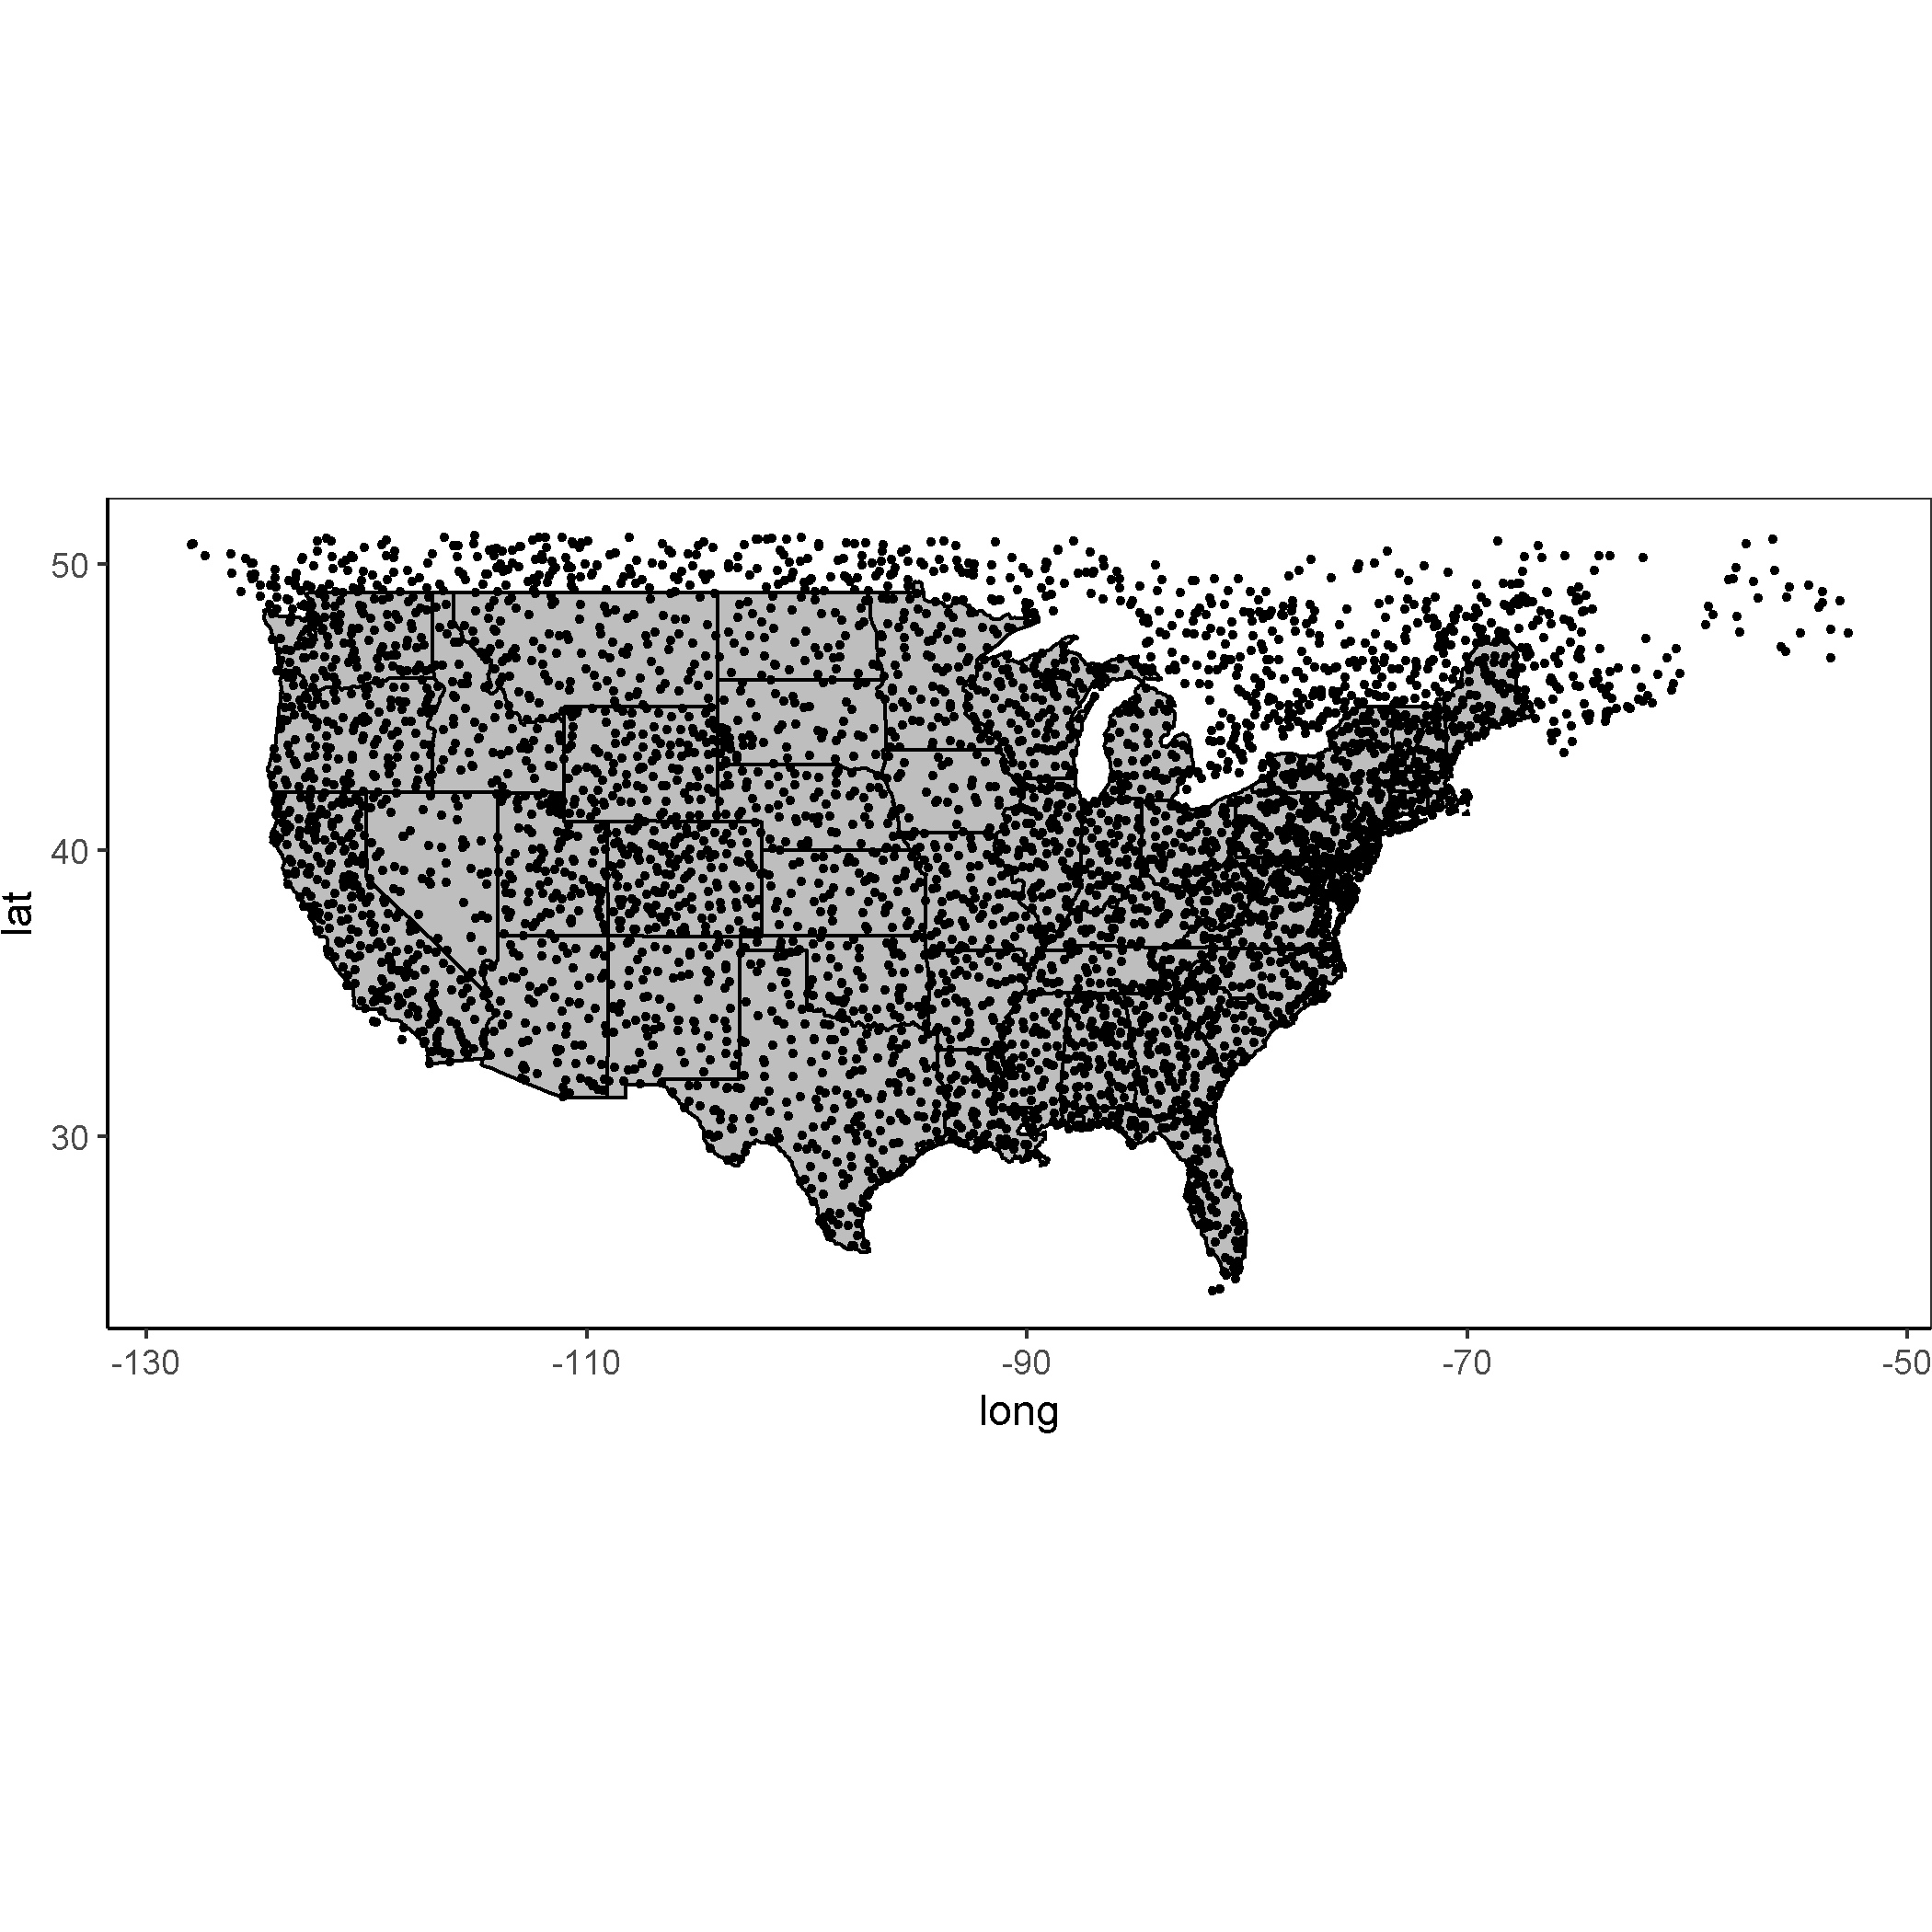
\includegraphics[width=0.95\linewidth]{./chapterFiles/fisherSpatial/figures/figsCalledInDiss/bbsRoutesUsed} \caption{Locations of Breeding Bird Survey routes sampled between 1966 and 2017.}\label{fig:bbsPoints}
\end{figure}
\subsection{Study area}\label{study-area}

Although the NABBS conducts surveys throughout much of North America, I
limited analyses to the continental United States and parts of southern
Canada. NABBS coverage of the boreal forests of Canada are sparse in
space, and many routes in Mexico have fewer than 25 years of
observations.
\begin{figure}
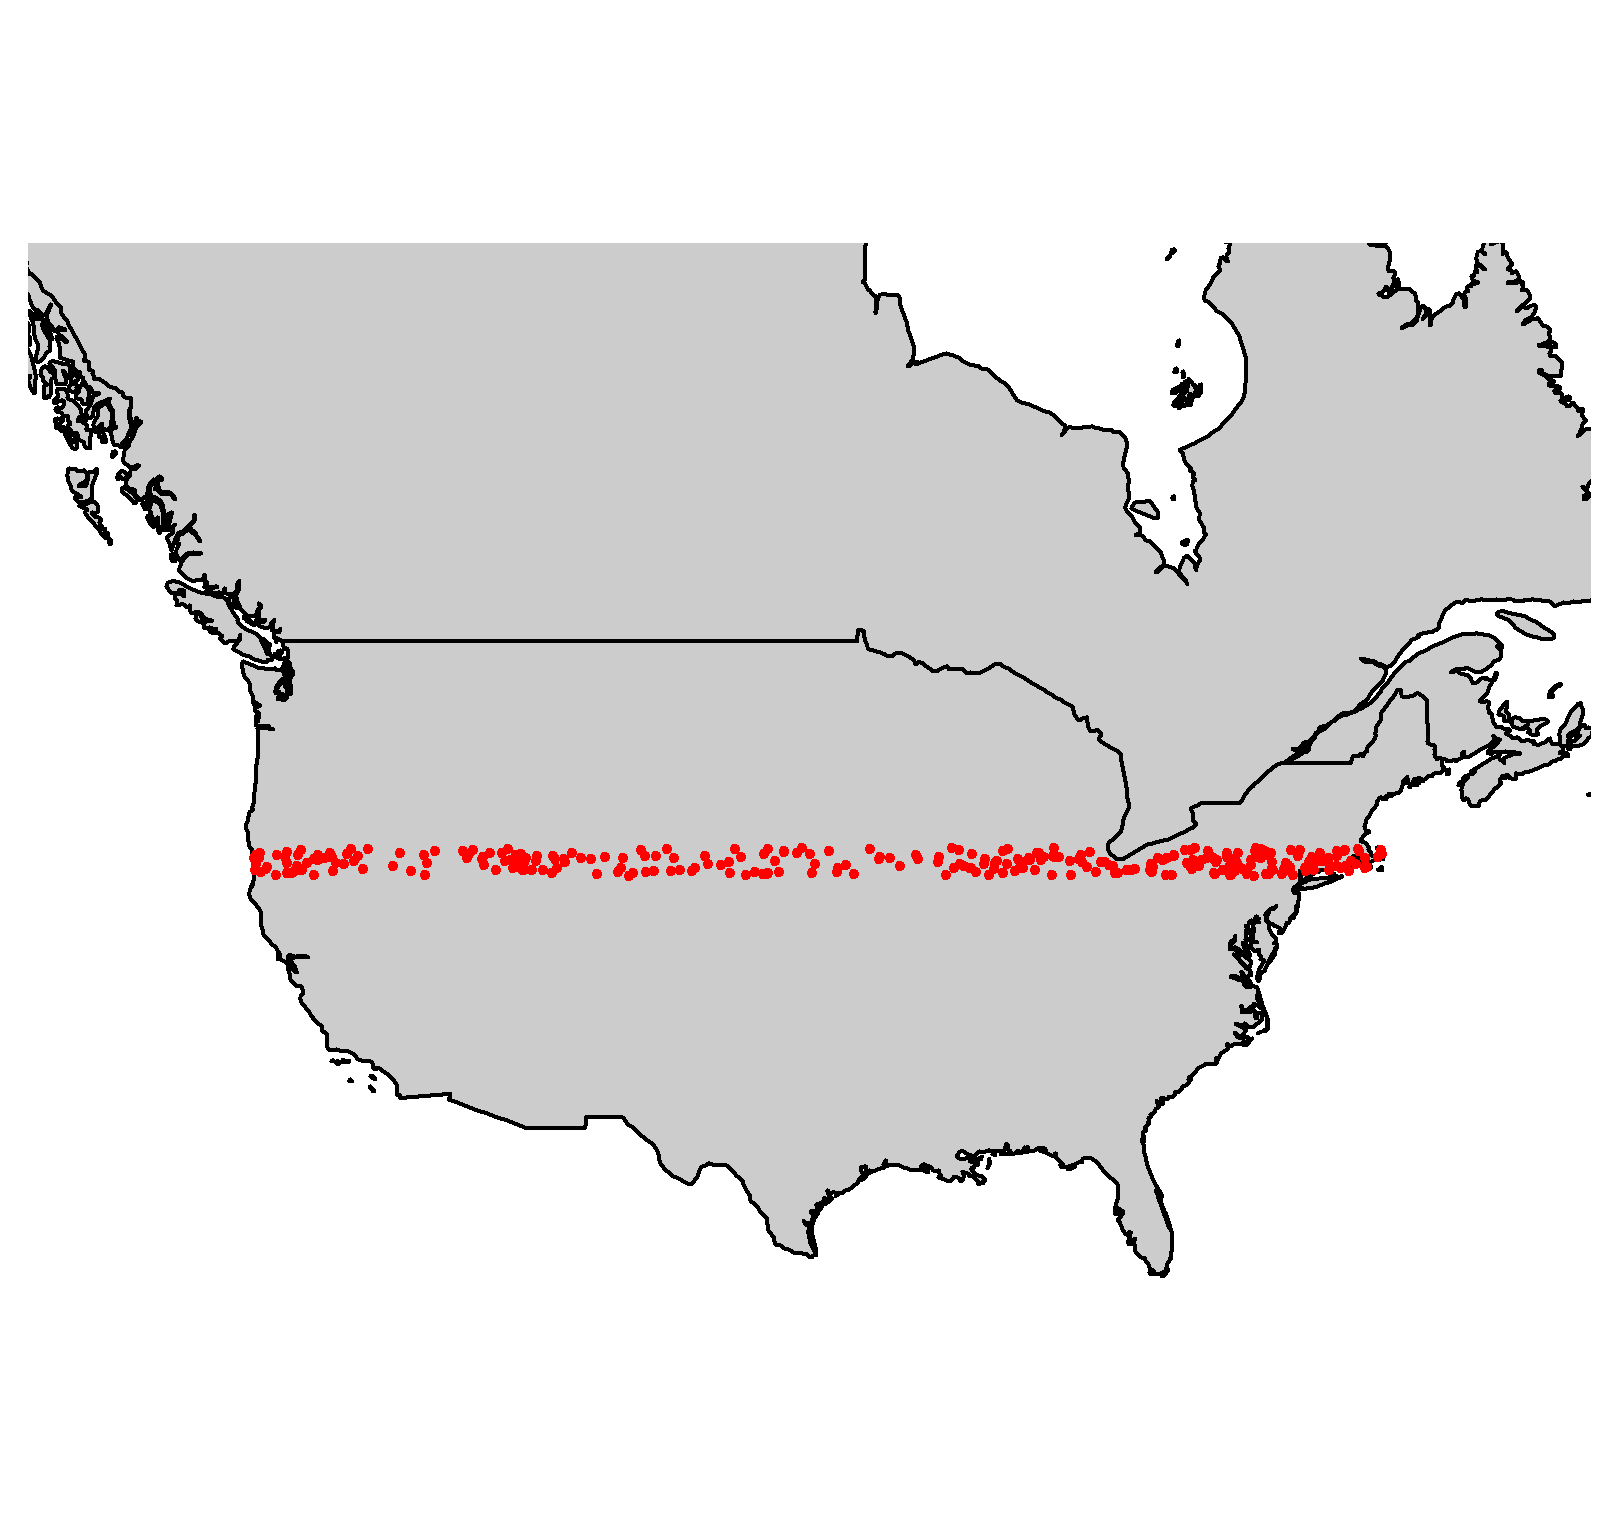
\includegraphics[width=0.95\linewidth]{./chapterFiles/fisherSpatial/figures/figsCalledInDiss/transectSamplingEx_1row} \caption{A single East-West transect of Breeding Bird Survey routes used to calculate the Fisher Information.}\label{fig:ewRouteMap}
\end{figure}
\subsubsection{Focal military base}\label{focal-military-base}

The Mission of the US Department of Defense is to provide military
forces to deter war and protect the security of the country, and a
primary objective of individual military bases is to maintain military
readiness. To maintain readiness, military bases strictly monitor and
manage their natural resources. Military bases vary in size and nature,
and are heterogeneously distributed across the continental United States
(See Fig. \ref{fig:ewRouteMap}). The spread of these bases (Fig.
\ref{fig:milBases}), coupled with the top-down management of base-level
natural resources presumably influences the inherent difficulties
associated with collaborative management within and across military
bases and other natural resource management groups (e.g., state
management agencies, non-profit environmental groups.

Much like other actively managed landscapes, miltiary bases are
typically surrounded by non- or improperly-managed lands. Natural
resource managers of military bases face environmental pressures within
and surrounding their properties, yet their primary objectives are very
different. Natural resource managers of military bases, whose primary
objective is to maintain military readiness, are especially concerned
with if and how broad-scale external forcings might influence their
lands. Prominent concerns include invasive species, wildlife disease,
and federally protected species (personal communication with Department
of Defense natural resource managers at Eglin Air Force and Fort Riley
military bases). For these reasons, natural resource managers attempt to
create buffers along their perimeters (e.g., live fire/ammunitions
suppression, wide fire breaks). Identifying the proximity of military
bases to historic and modern ecological shifts may provide insight into
the effectiveness of their natural resource management efforts.
\begin{figure}

{\centering 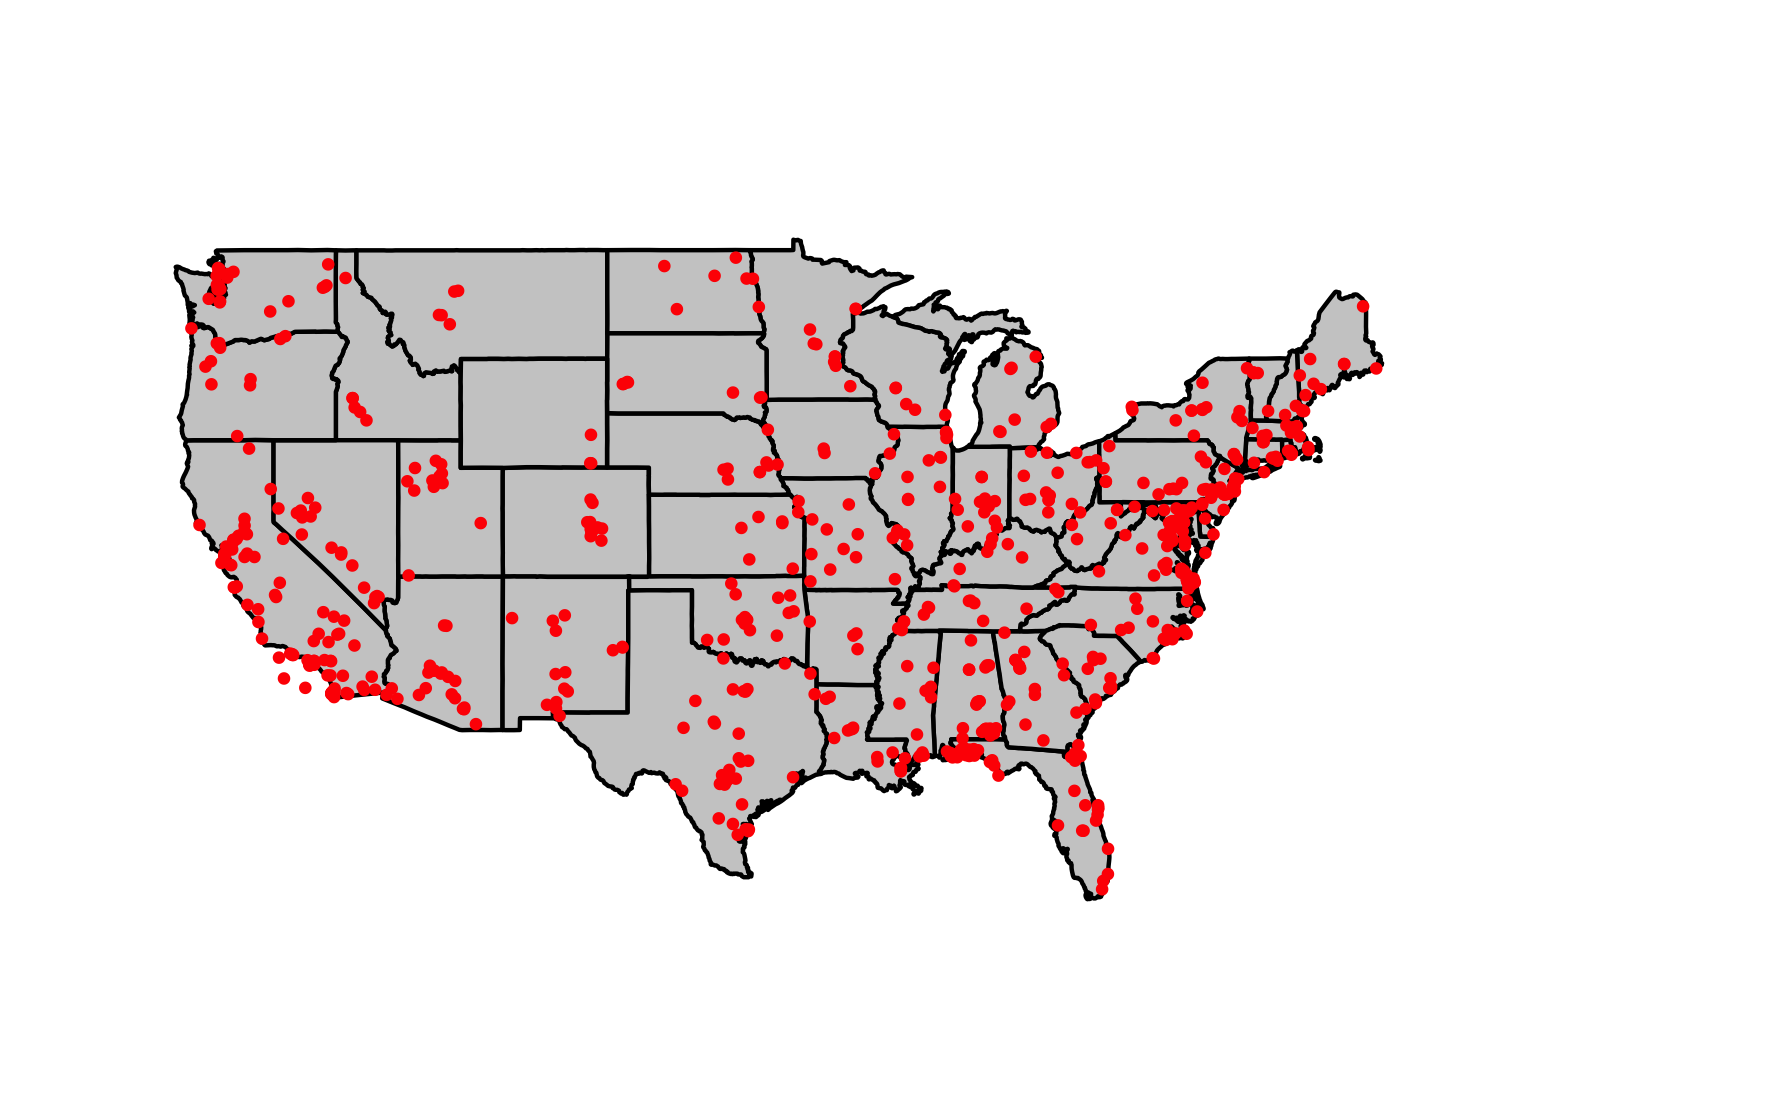
\includegraphics[width=0.95\linewidth]{./chapterFiles/fisherSpatial/figures/figsCalledInDiss/milBases} 

}

\caption{Locations of U.S. military bases in our study area.}\label{fig:milBases}
\end{figure}
The NABBS routes chosen for analyses in this Chapter lie within or near
Fort Riley military base (located at approximately
\(39.110474^{\circ}\), \(-96.809677^{\circ}\); Kansas, USA). Fort Riley
(\ref{fig:basesOfInterestMap}) is a useful reference site for this
study. Woody encroachment of the Central Great Plains over the last
century has triggered shifts in dominant vegetative cover and diversity
(Ratajczak et al. 2012) in the area surrounding Fort Riley military base
(e.g., Van Auken 2009). This phenomena should present itself as a regime
boundary should Fisher Information be a robust regime shift detection
method.
\begin{figure}

{\centering 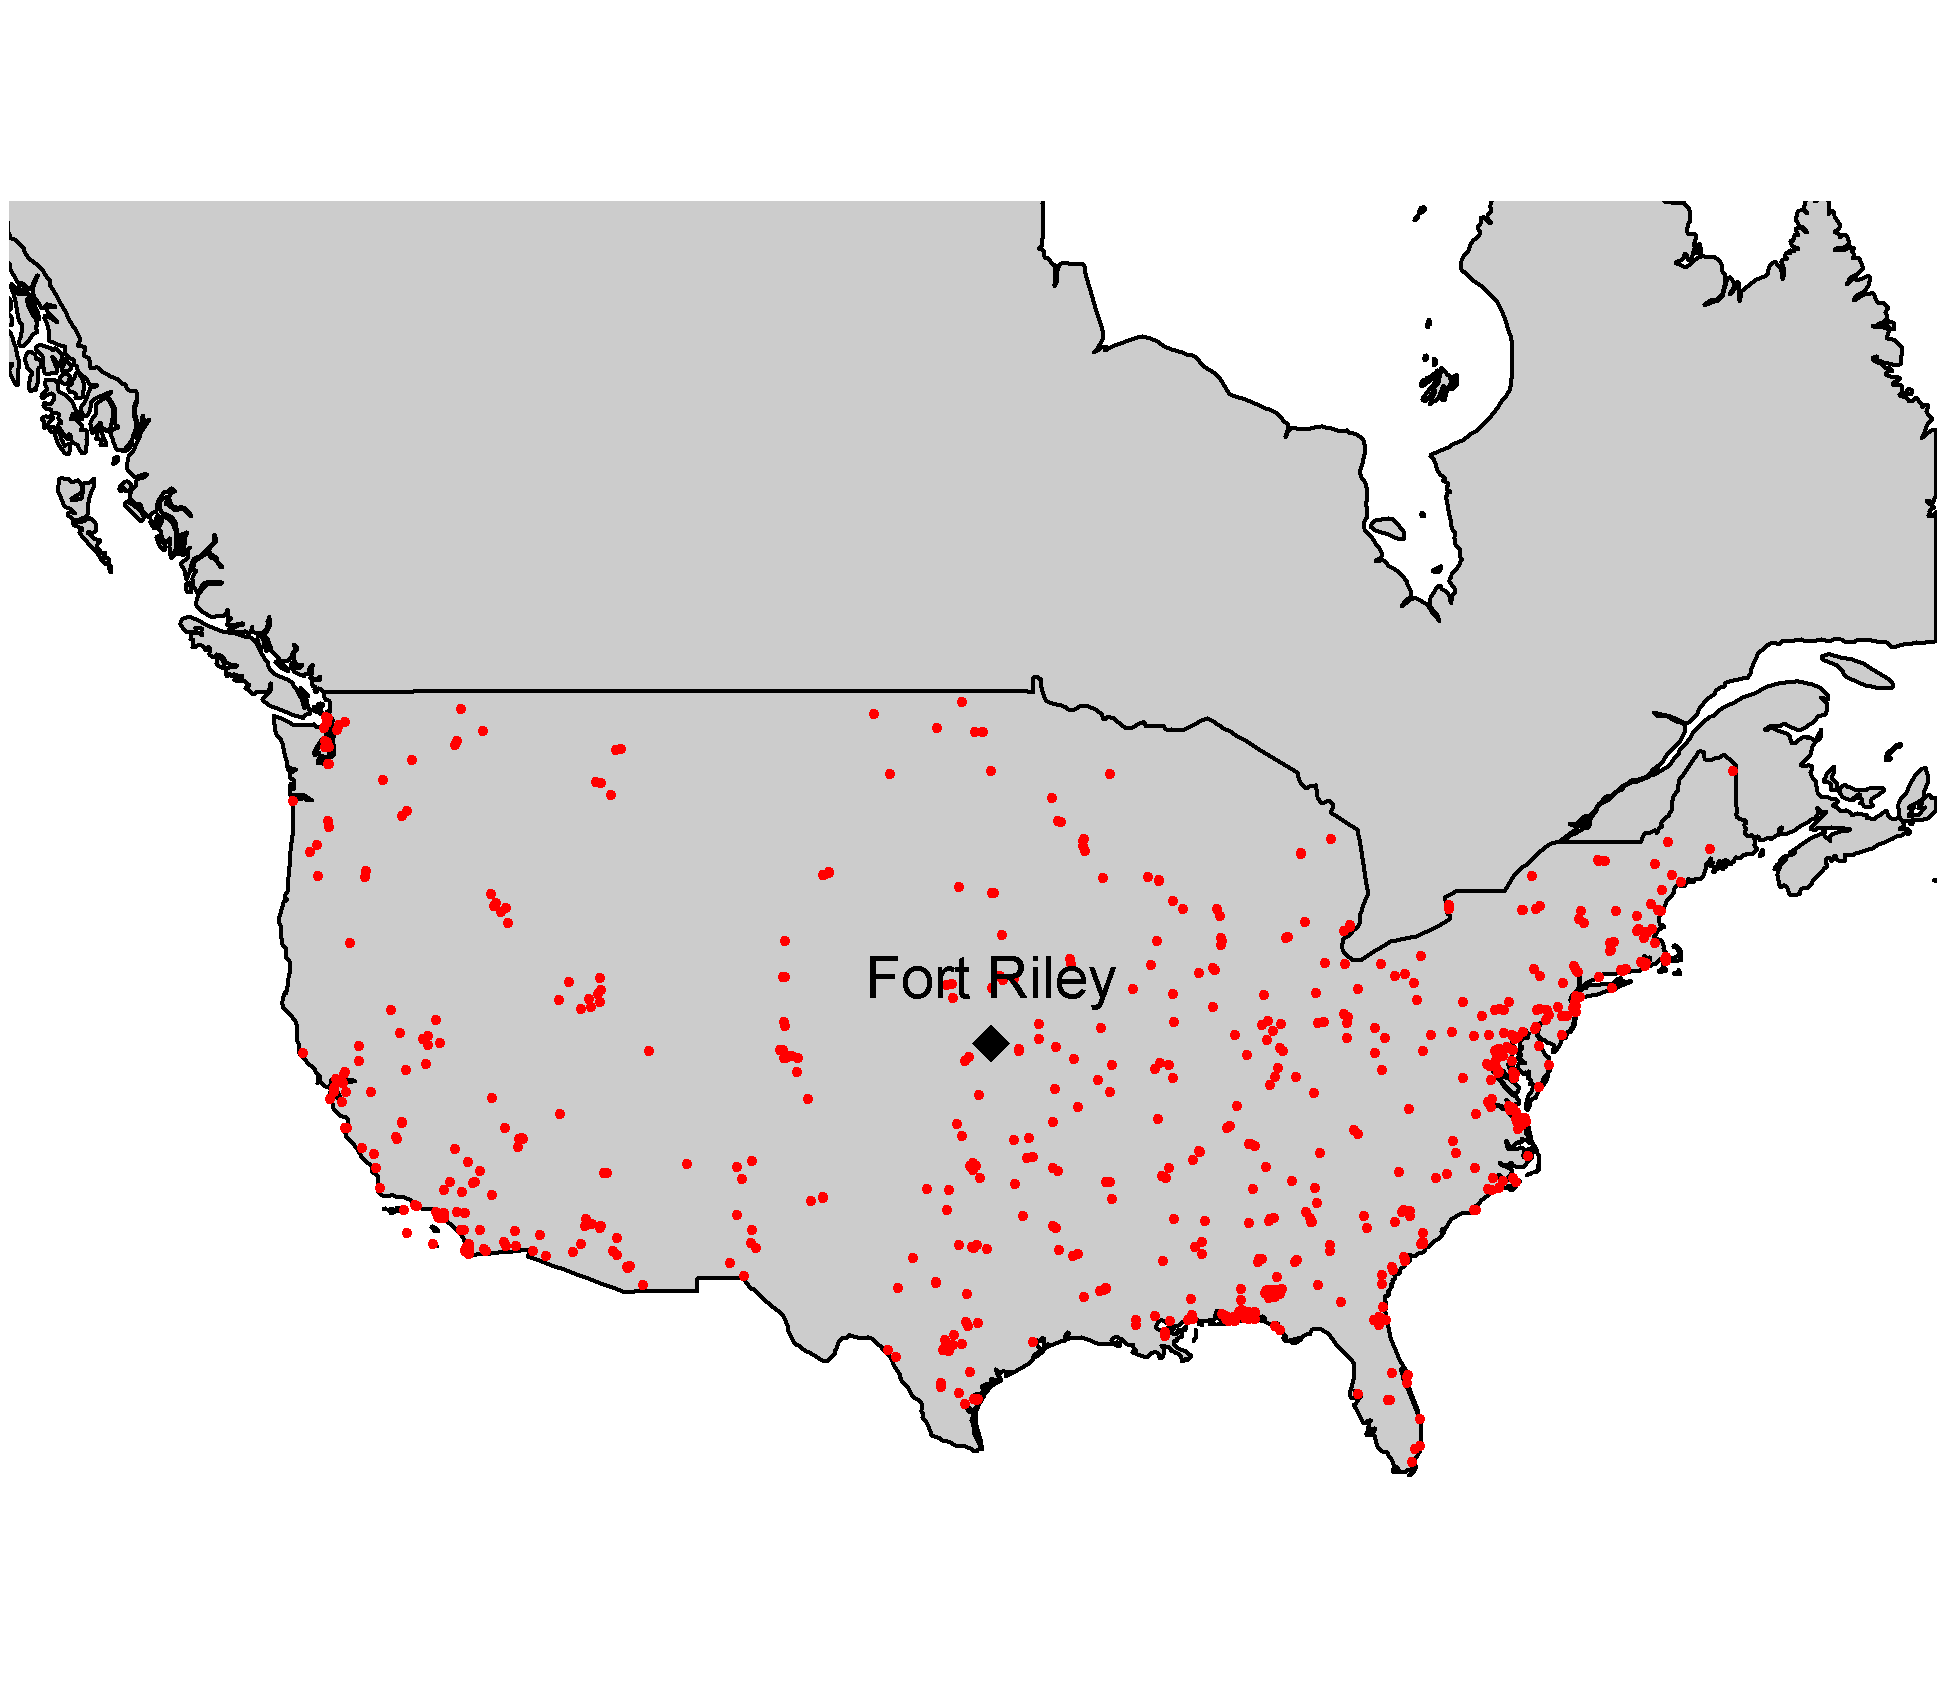
\includegraphics[width=0.95\linewidth]{./chapterFiles/fisherSpatial/figures/figsCalledInDiss/basesOfInterestMap} 

}

\caption{Locations of focal U.S. military bases, Eglin Air Force Base (AFB) and Fort Riley Military Base.}\label{fig:basesOfInterestMap}
\end{figure}
\subsubsection{Spatial sampling grid}\label{spatial-sampling-grid}

To my knowledge, Sundstrom et al. (2017a) is the only study to use the
Fisher Information on spatially-referenced data. The authors of this
study hand-picked NABBS routes to be included in their samples such that
their metrics should detect `regime changes' when adjacent sampling
points represented different ecoregions (broad-scale vegetation
classification system). The authors also suggest each ecoregion is
similarly represented, having a similar number of NABBS routes within
each ecoregion in the analysis. However, this method of handpicking
routes resulted in a transect which was neither North-South nor
East-West running (see Sundstrom et al. (2017a)), but rather zigzagged
across a midwestern region.
\begin{figure}

{\centering \includegraphics[width=0.95\linewidth]{./chapterFiles/fisherSpatial/figures/figsCalledInDiss/transectSamplingALlRoutesUsed} 

}

\caption{The five East-West running transects used to visualize results in this chapter.}\label{fig:ewRoutesUsedHere}
\end{figure}
I constructed a gridded system across the continental United States and
parts of Canada. The gridded system comprises East-West running
transects transects running in either North-South or East-West
directions. This method ameliorates some sampling bias, as I have
arbitrarily defined sampling transects, rather than hand-picking sites
to include in the analysis. Additionally, this approach allows for
raster stacking, or layering data layers (e.g., vegetation, LIDAR,
weather) on top of the sampling grid and results, allowing one to
identify potential relationships with large-scale drivers. This method
also provides a simple vector for visualizing changes in the Fisher
Information over space-time, using animations and still figures. For
brevity, I present visual results of only five, spatially-adjacent,
East-West running transects (Fig. \ref{fig:ewRoutesUsedHere}) at
multiple time periods.

\subsection{Fisher Information (FI)}\label{fisher-information-fi}

Fisher Information, \(I(\theta)\), was developed in 1922 by Ronald
Fisher as a measure of the amount of information that an observable
variable, X, reveals about an unknown parameter, \(\theta\). Fisher
Information is a measure of indeterminacy (Fisher 1922) and is defined
as,
\begin{equation} 
  I(\theta) = \int \frac{dy}{p(y|\theta)}\left[\frac{dp(y|\theta)}{d\theta}\right]^2
  \label{eq:fiGeneral1922}
\end{equation}
where \(p(y|\theta)\) is the probability density of obtaining the data
in presence of \(\theta\). The Fisher Information measure (FIM) is used
to calculate the covariance matrix associated with the likelihood,
\(p(y|\theta)\). Fisher Information is described as Extreme Physical
Information (EPI; Frieden and Soffer 1995, Kibble 1999, Frieden et al.
2002), a measure that has been used to track the complexity of systems
in many scientific disciplines including, physics, cancer research,
electrical engineering, and, recently, complex systems theory and
ecology

Fisher Information as gathered from observational data provides insight
as to the dynamic order of a system, where an orderly system is one with
constant (i.e., unchanging) observation points, and one whose nature is
highly predictable. A disorderly system is just the opposite, where each
next data point is statistically unpredictable. In ecological systems,
patterns are assumed to be a realization of ecosystem order; therefore,
oneshould expect orderliness in a system with relatively stable
processes and feedbacks. Orderliness, however, does not necessarily
infer long-term predictability. \eqref{eq:fiGeneral1922} is next adapted
to estimate the dynamic order of an entire system, \(s\), as
\begin{equation} 
  I = \int \frac{ds}{p(s)}\left[\frac{dp(s)}{ds}\right]^2
\end{equation}
where \(p(s)\) is the probability density for \(s\). Here, a relatively
high Fisher Information value (\(I\)) infers higher dynamic order,
whereas a lower value (approaching zero) infers less orderliness. To
limit the potential values of \(I\) in real data, we can calculate the
amount of Fisher Information by re-expressing it in terms of a
probability amplitude function \(q(s)\) (Fath et al. 2003, Mayer et al.
2007, eq. 7.3):
\begin{equation}
  I = 4 \int ds\left[\frac{dq(s)}{ds}\right]^2
  \label{eq:fiAmplitude}
\end{equation}
A form specific to the pdf of distance travelled by the entire system,
which I call the `derivatives' method, is defined as (D. A. L. Mayer,
Pawlowski, Fath, \& Cabezas, 2007, eq. 7.12):
\begin{equation}
  I = \frac{1}{T} \int_0^T dt\left[\frac{s''^2}{s'^4}\right]^2
  \label{eq:fiDerivs}
\end{equation}
where T is the number of equally spaced time points over which the data
are integrated. Numerical calculation of \(I\) using the binning method
(Eq. \eqref{eq:fiAmplitude} and \eqref{eq:derivativesFI}) each incorporate a
moving-window procedure for calculating the probability of the system,
\(p(s)\), as being in one of an unidentified number of states (\(s\)).
Although previously applied to spatially-explicit terrestrial community
data,the binning method (Eq. \ref{derivatives}) requires multiple
parameters to be defined \emph{a priori}, which have been shown to
influence inference based on the metric. I therefore calculated FI using
the derivatives equation (Eq. \ref{fiDerivs}).

The binning procedure allows for a single point in time or space to be
categorized into more than one state, which violating the properties of
alternative stable states theory. The size of states (see Eason and
Cabezas 2012) measure is required to construct p(s). In the case of high
dimensional data, a univariate binning procedure of p(s) is not
intuitive (i.e., reducing a multivariable system to a single probability
distribution rather than constructing a multivariate probability
distribution). Importantly, when using community or abundance data, rare
or highly abundant species can influence the size of states criterion,
thus influencing the assignment of each point into states. Finally, Eq.
\eqref{eq:fiAmplitude} assumes equal spacing (in space or time) between
sampling points. Each of these violations can be avoided by using Eq.
\eqref{eq:fiDerivs}; Cabezas and Fath 2002, Fath et al. 2003) to calculate
the Fisher Information measure (see Chapter @derivatives for discussion
on this topic). The derivatives method (Eq. \eqref{eq:fiDerivs}) estimates
the trajectory of the system's state by calculating the integral of the
ratio of the system's acceleration and speed in state space (B. D. Fath,
Cabezas, \& Pawlowski, 2003). I calculated FI using Equation
\eqref{eq:fiDerivs} for every South-North and East-West transect (see
Figs. \ref{fig:bbsPoints}, \ref{fig:ewRoutesUsed}) for every year
between 1975 and 2018. \#\#\#\# Interpreting FI Here I define a
potential regime change or spatial regime as a point(s) exhibiing a
relatively large change in the Fisher Information value and having a
non-zero first derivative. Regime shifts are identified as data changing
from one state to another, thus, rapid shifts in the value of FI should
indicate the points, in time or space, at which the system undergoes
reorganization. Spatial and temporal Fisher Information calculation does
not vary, but interpretation of either differ in that a spatial analysis
will identify a spatial regime boundary (Sundstrom et al., 2017a) in
space within a single time period, whereas analysis of temporal data
will identify a point(s) in time at which a system in a specific
location undergoes a regime shift. I follow the methods outlined in the
relevant literature for interpreting the Fisher Information (e.g.,
Karunanithi, Cabezas, Frieden, \& Pawlowski, 2008, Eason \& Cabezas
(2012)).

Increases in FI is supposed to indicate an increase in system
orderliness, where periods of relatively high values of I as the system
occurring in a single state, or fluctuating around a single attractor. A
rapid change in FI is supposed to indicated the system is no longer
orderly and may be undergoing a reorganization phase. Whether Fisher
Information can identify a switch among basins of attraction within a
single, stable state (or around a single attractor) remains unknown, as
does the number of states which a system can occupy. When a system
occurs within any number of states equally, i.e., p(s) is equal for each
state, both the derivative, (\(\frac{dq(s)}{ds}\), and \(I\) are zero.
As \((\frac{dq(s)}{ds} \rightarrow \infty)\), we infer the system is
approaching a stable state, and as \(\frac{dq(s)}{ds} \rightarrow 0\)
the system is showing no preference for a single stable state and is on
an unpredictable trajectory. \eqref{eq:fiAmplitude} bounds the potential
values of Fisher Information at \([0, 8]\), whereas
\eqref{eq:fiGeneral1922}, \eqref{eq:fi73c}, and \eqref{eq:derivativesFI} have
are positively unbounded \([0, \infty)\). If the Fisher Information is
assumed to represent the probability of the system being observed in
some state, \(s\), then the absolute value of the Fisher Information
index is relative within a single datum (here, transect). It follows
that Fisher Information should be interpreted relatively, but not
absolutely.

\subsection{Efficacy of Fisher Information as a spatial
RDM}\label{efficacy-of-fisher-information-as-a-spatial-rdm}

Rapid changes in either direction of Fisher Information is suggested to
indicate of a regime shift (A. L. Mayer, Pawlowski, \& Cabezas, 2006,
({\textbf{???}}) 2012). Although this interpretation has been applied to
multiple case studies of Fisher Information, there is yet a statistical
indicator to objectively identify these abrupt changes.

After calculating the Fisher Information for each spatial transect (Fig.
\ref{fig:ewRoutesUsedHere}) during each sampling year, I used pairwise
correlation to determine whether spatial autocorrelation existed among
pairs of spatial transects. If some set of points, \(N\), are close in
space and are \emph{not} separated by some physical or functional
boundary (e.g., an ecotone, a river), then they should exhibit some
degree of spatial autocorrelation. It follows that the correlation
coefficient of spatially adjacent transects should be similar, diverging
only as the distance beteween the transects differs and/or a functional
or physical boundary separates them.

\subsubsection{Linear interpolation of Fisher
Information}\label{linear-interpolation-of-fisher-information}

Because the BBS routes are not regularly spaced, pairwise correlations
of adjacent transects are not possible without either binning the Fisher
Information calculations, or interpolating the results to
regularly-spaced positions in space. I linearally interpolated Fisher
Information within each spatial transect (Fig.
\ref{fig:ewRoutesUsedHere}) at 50 points along the longitudinal axis.
The 50 longitudinal points at which I interpolated were the same across
each spatial transect. I used the function \texttt{stats::approx()} to
linearly approximate the Fisher Information. I did not interpolate
values beyond the longitudinal range of the original data
(\texttt{rule=1}).

\subsubsection{Correlation of Fisher Information among adjacent spatial
tranects}\label{correlation-of-fisher-information-among-adjacent-spatial-tranects}

I calculate the pairwise correlation (Pearson's) among each pair of
adjacent spatial transects (e.g., Fig. \ref{fig:adjacentTsectEx}) using
the function \texttt{stats::cor()}. I removed a pair of points if at
least one point was missing an estimate for Fisher Information. This
occurred when the original longitudinal range of one transect exceeded
its pair's range, since I did not interpolate beyond the original
longitudinal range.
\begin{figure}

{\centering 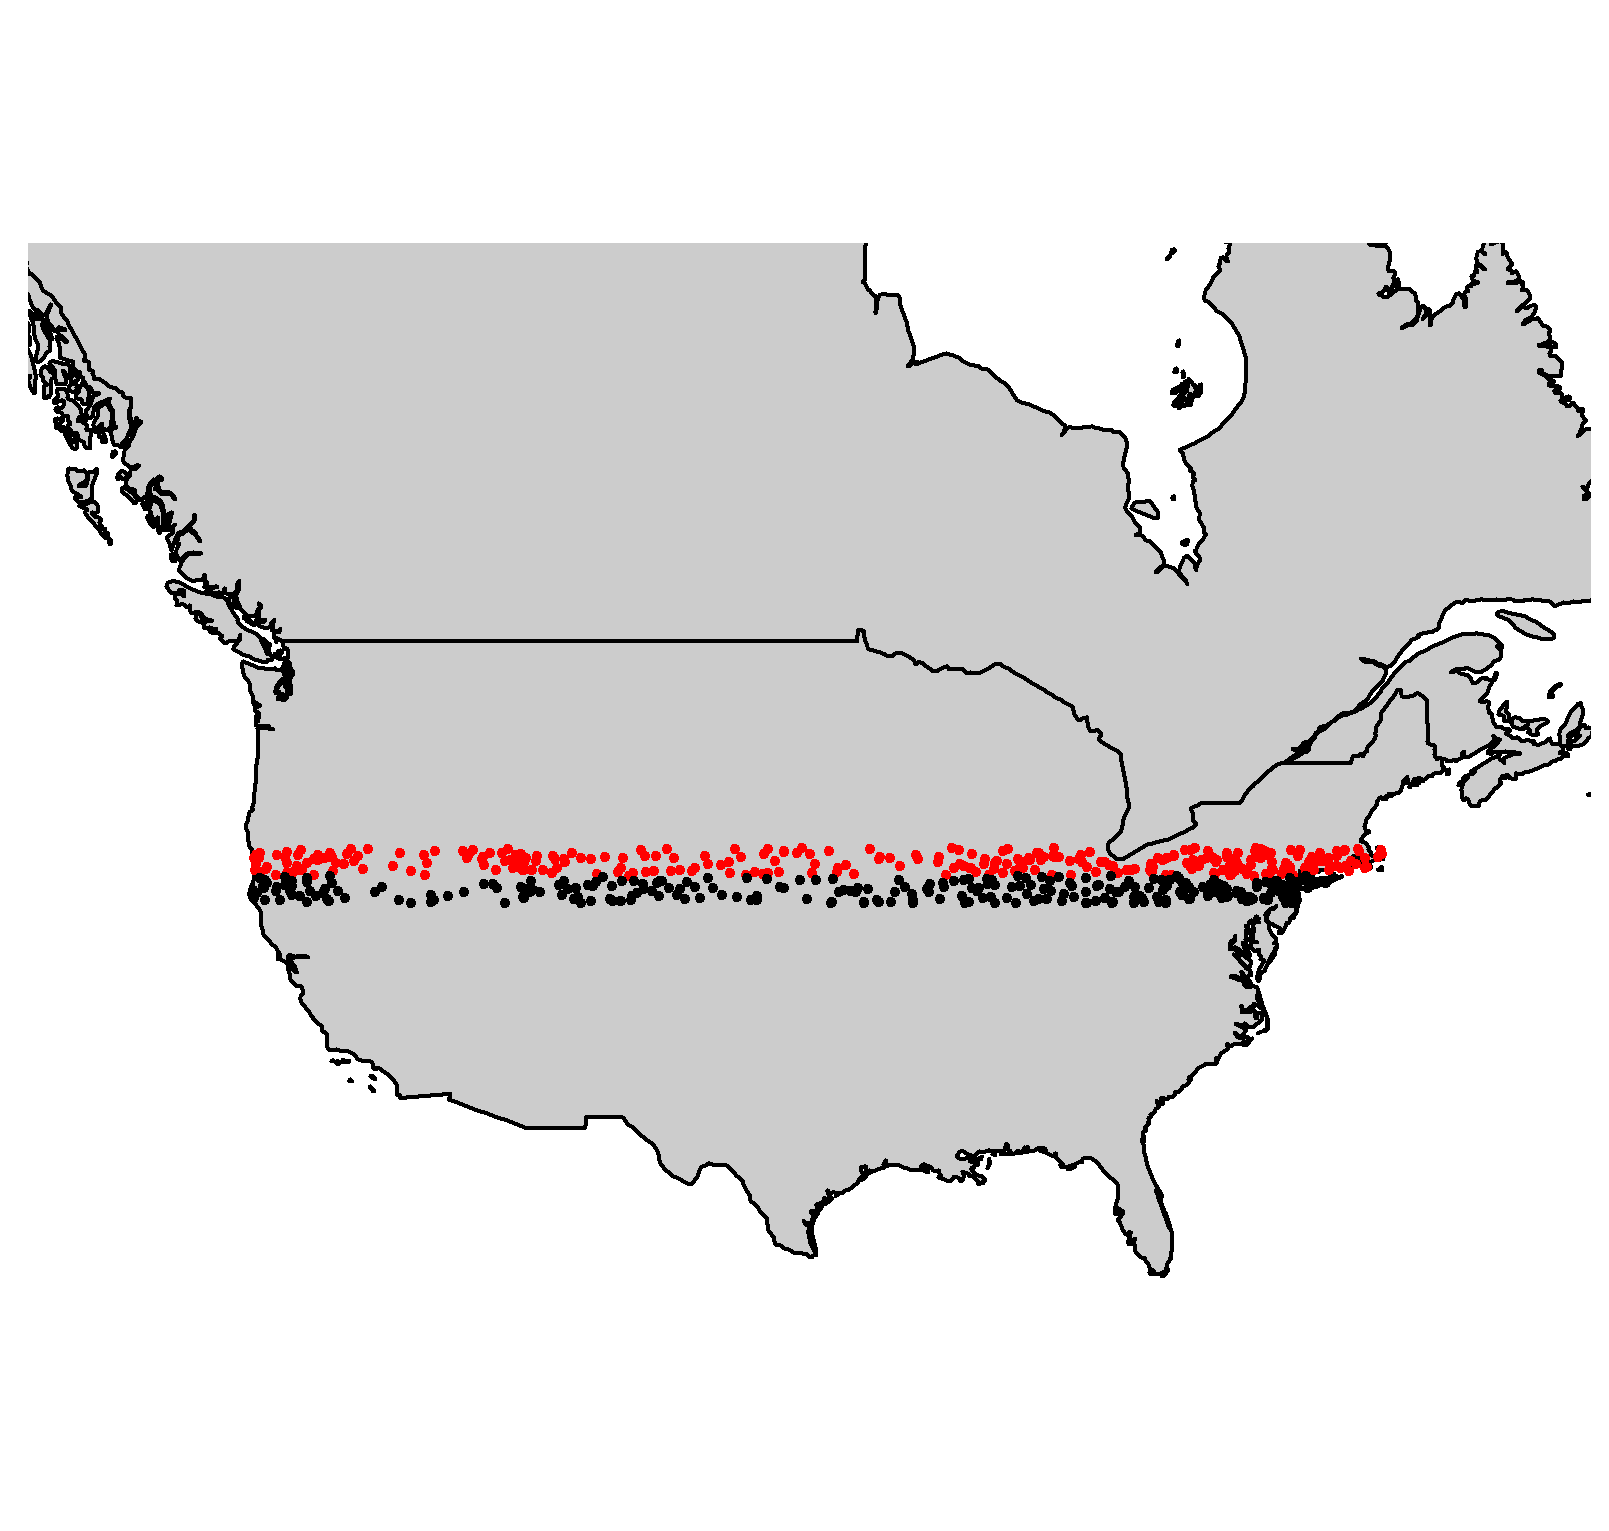
\includegraphics[width=0.95\linewidth]{./chapterFiles/fisherSpatial/figures/figsCalledInDiss/transectSamplingEx_2rows} 

}

\caption{An example of two adjacent spatial transects within my sampling grid. After Fisher Ifnomration was calculated within a single transect, correlations were then calculated to determine the relationship among transect-pairs.}\label{fig:adjacentTsectEx}
\end{figure}
\section{Results}\label{results-1}

\subsection{Fisher Information}\label{fisher-information}

Interpreting the Fisher Information is currently a qualitative effort.
As suggested earlier, rapid increases or decreases in FI are posited
indicate a change in system orderliness, potentially suggesting the
location of a regime shift. Using this method yields inconclusive
results regarding the location of `spatial regime shifts' (Fig.
\ref{fig:fi1Tsect}).

Of the five spatial transects analyzed in this chapter (Fig.
\ref{fig:ewRoutesUsedHere}), Fig.\ref{fig:fi1Tsect} is representative of
the FI values obtained for the remaining transects. There is no clear
pattern within or among spatial transects across space or time
(Fig.\ref{fig:usaFI}). Log-transforming the Fisher Information metric
suppresses some of the extreme values, but still does not help identify
locations of regime changes. No clear regime changes exist in areas
where we might expect rapid changes (e.g., along the 105th meridian
West, where a sharp change in altitude occurs).
\begin{figure}
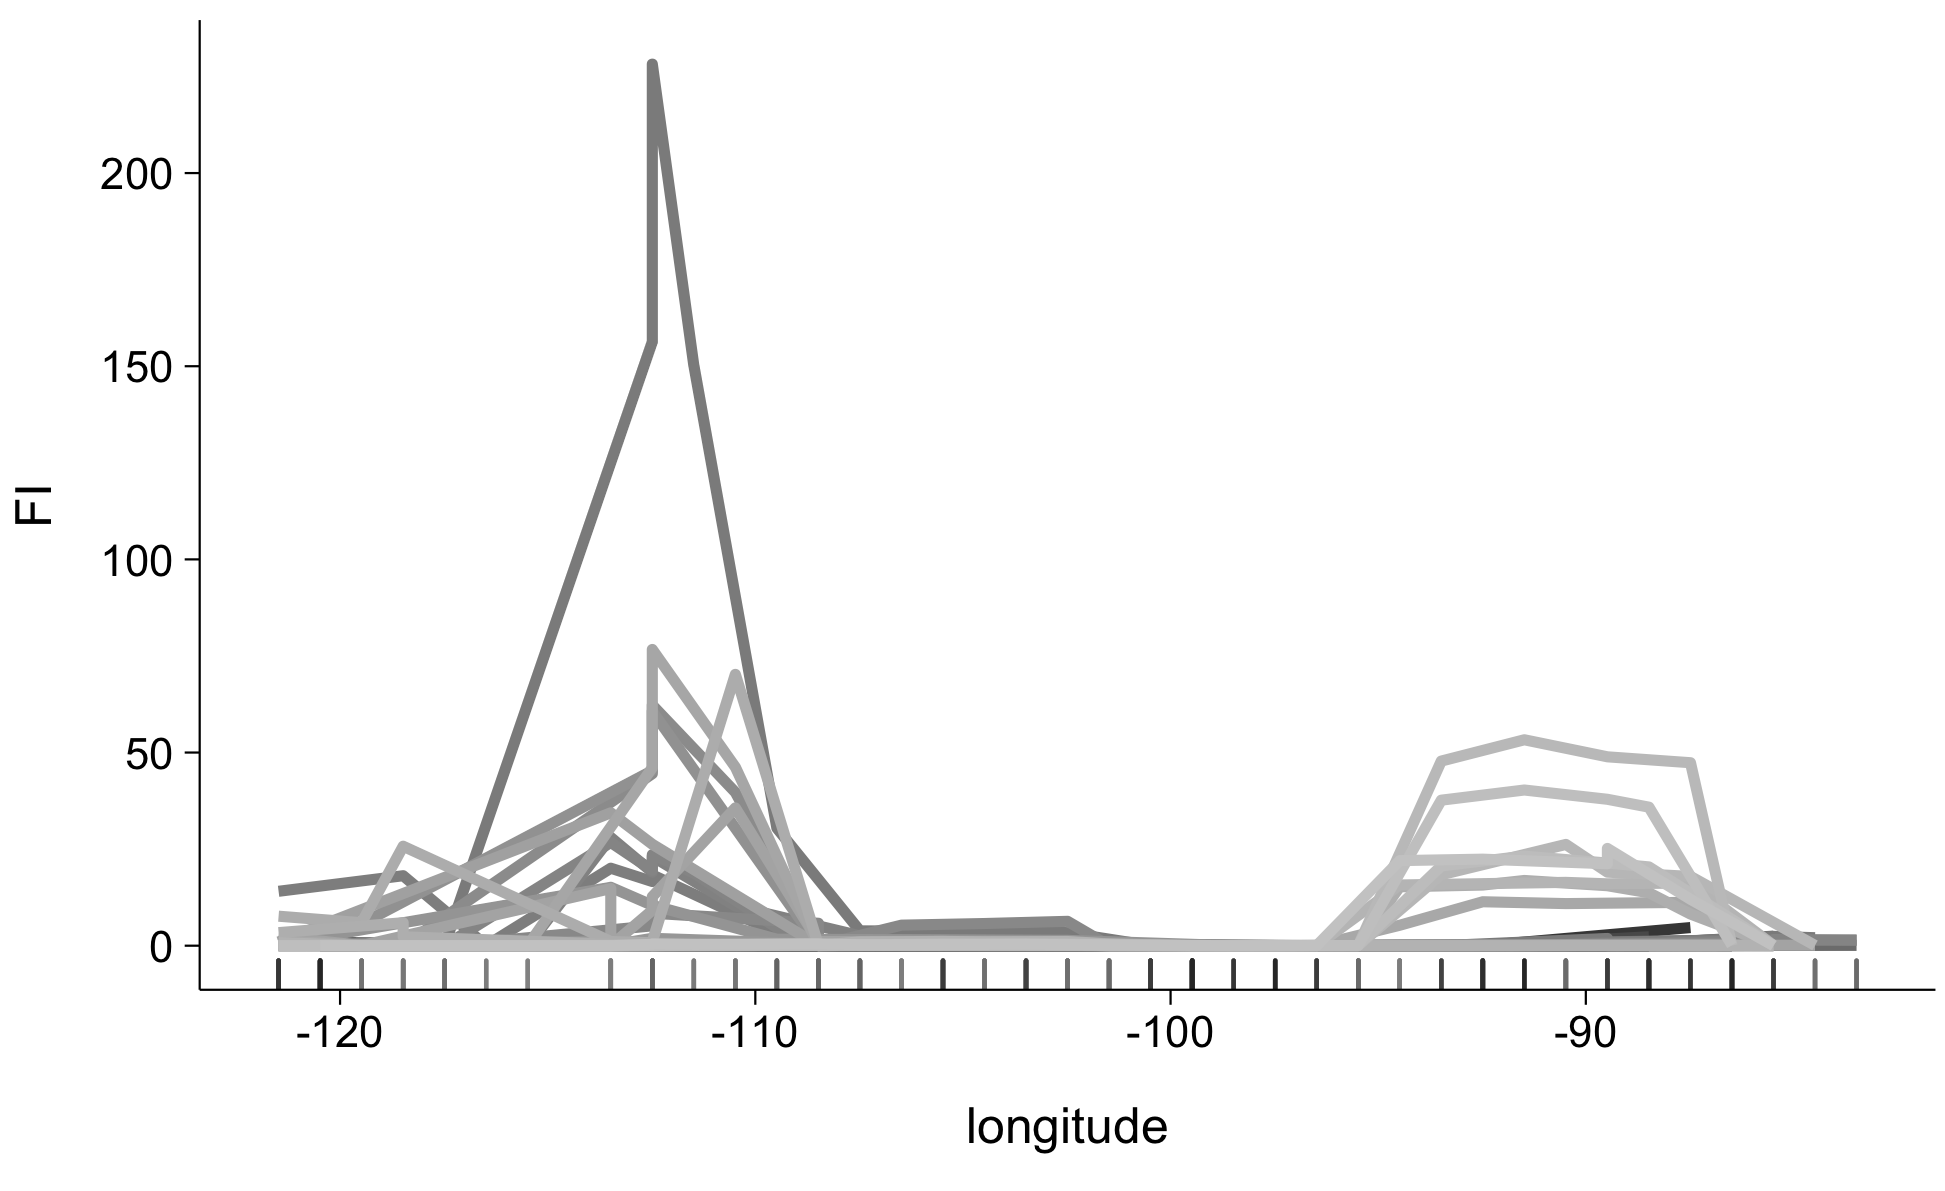
\includegraphics[width=0.95\linewidth]{./chapterFiles/fisherSpatial/figures/figsCalledInDiss/transect_15_East-West_metric_FI_Eqn712} \caption{Fisher Information calculated for a single transect (number 15) over time.}\label{fig:fi1Tsect}
\end{figure}
\begin{figure}
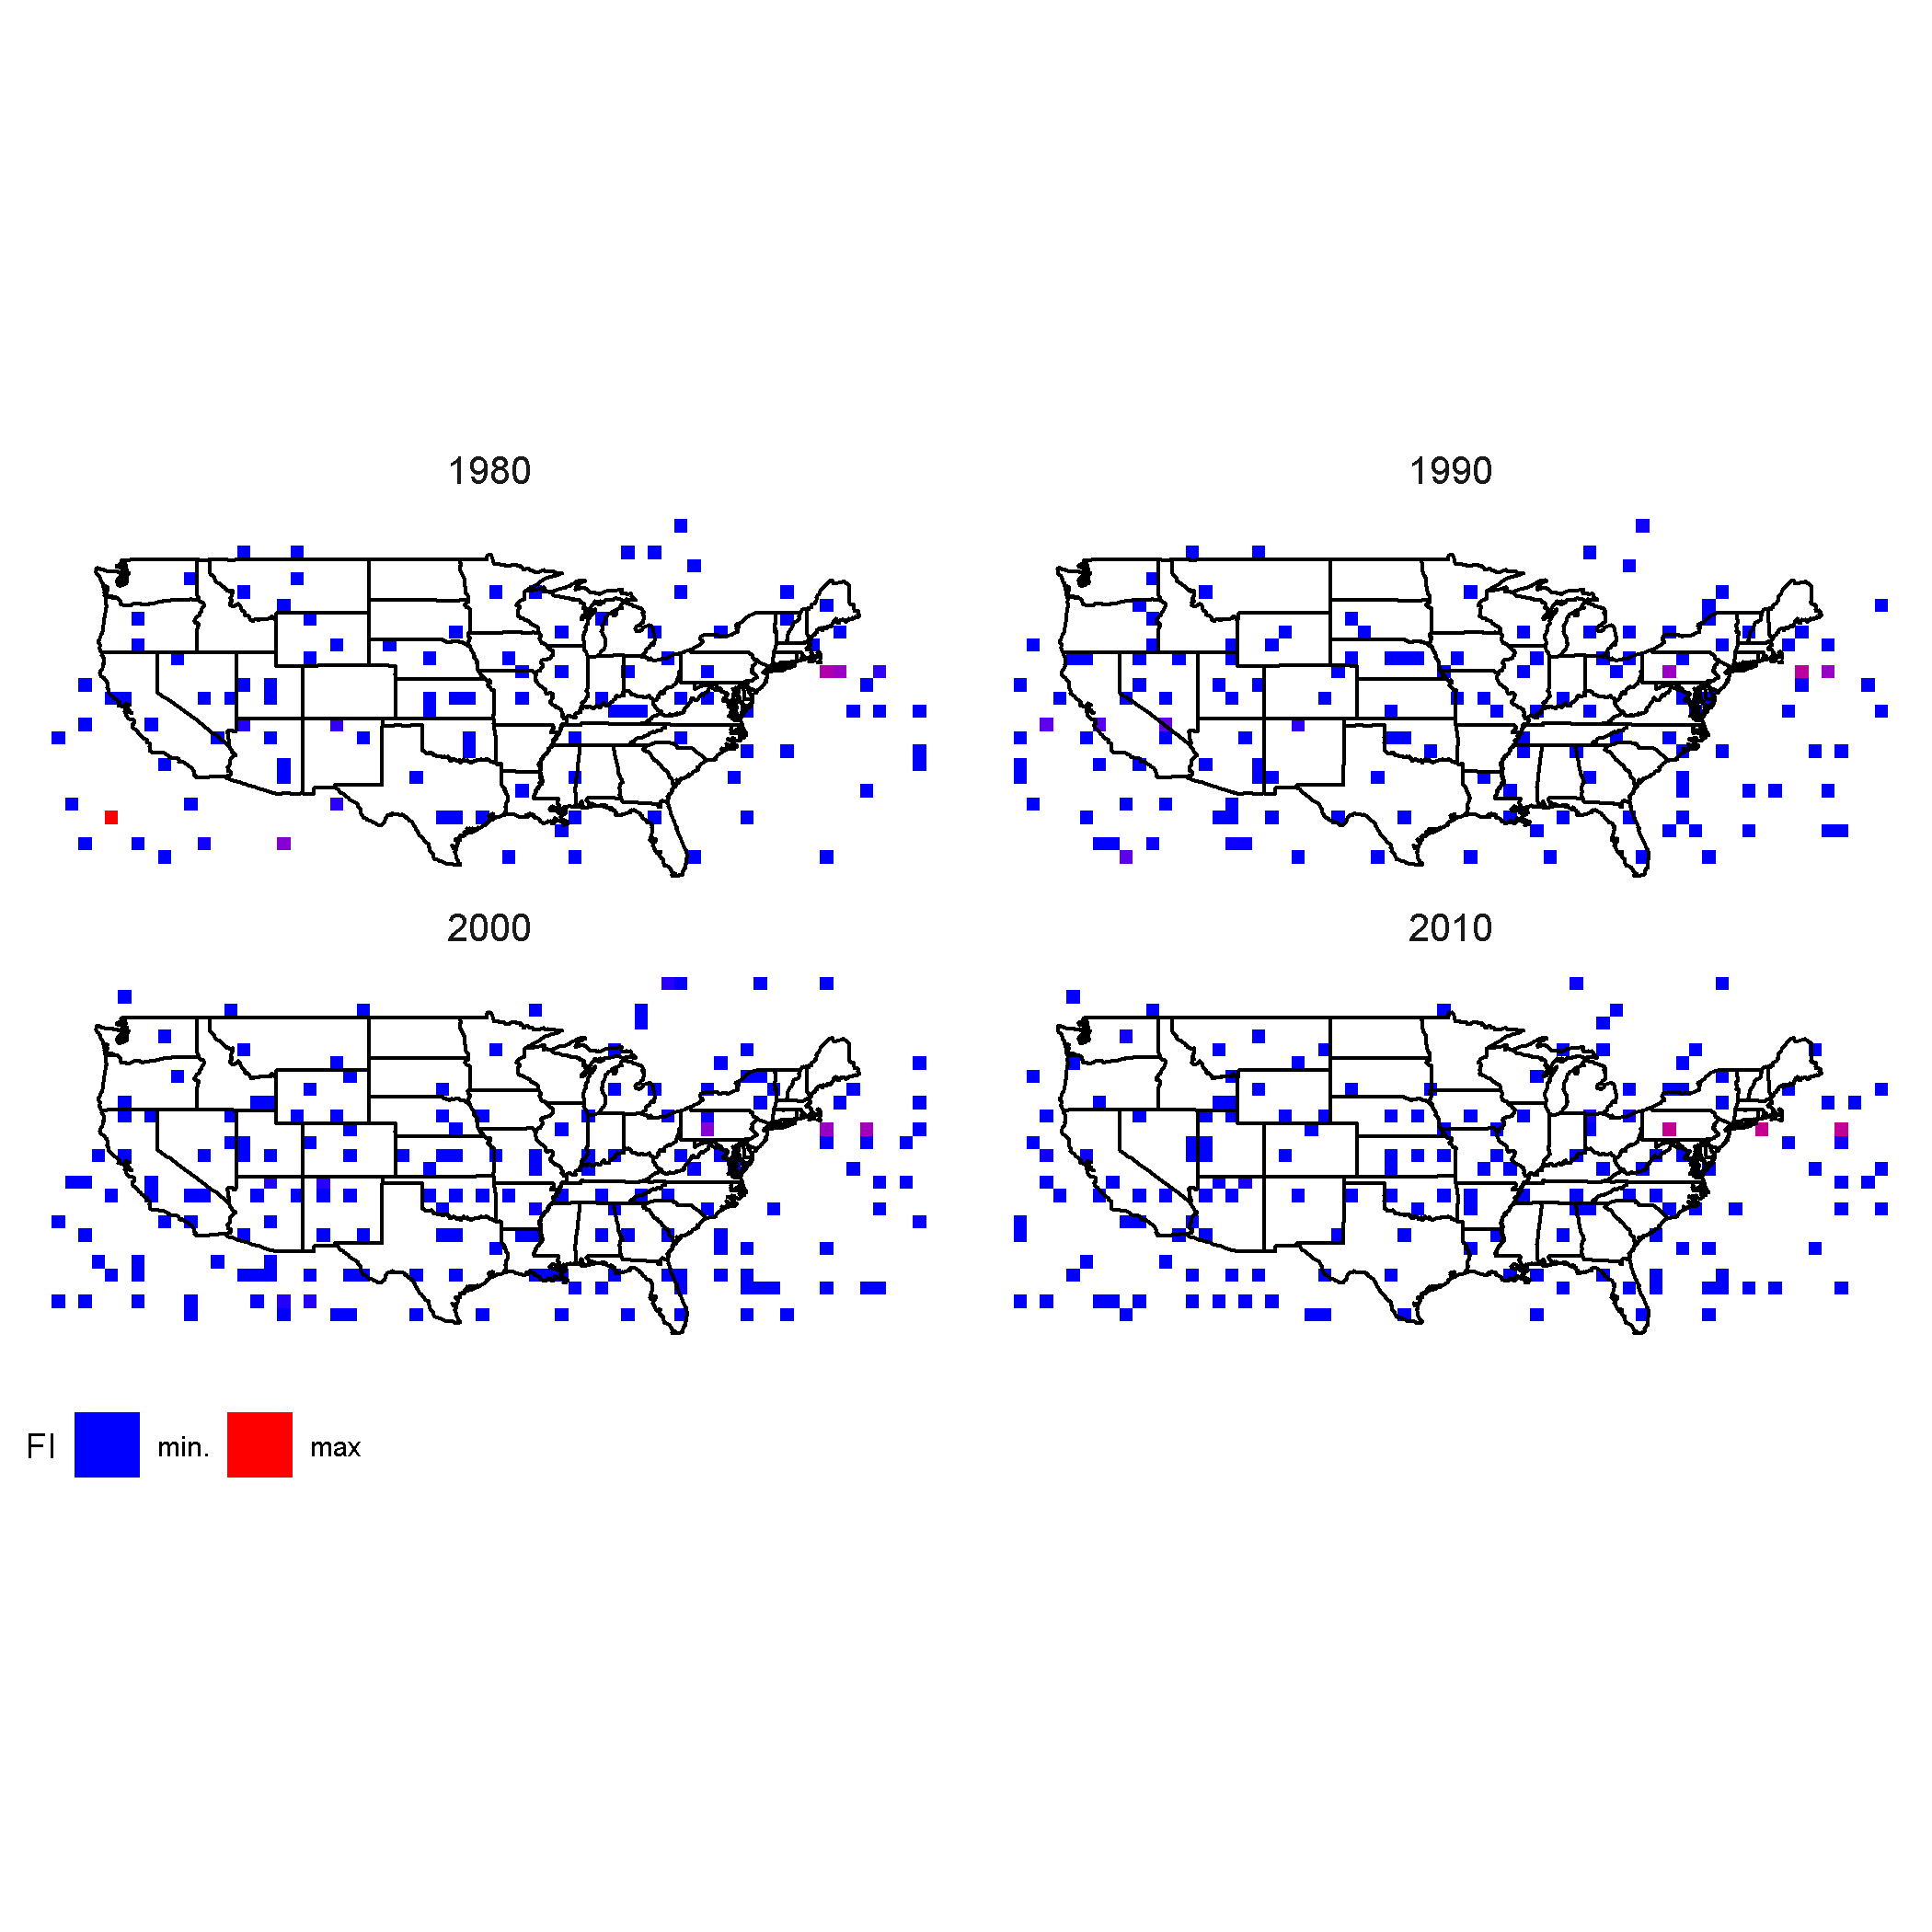
\includegraphics[width=0.95\linewidth]{./chapterFiles/fisherSpatial/figures/figsCalledInDiss/usaAllTsects_East-West_metric_FI} \caption{Fisher Information (top; log-scale bottom) of 5 East-West spatial transects over time. Adjacent changes of blue to red or vice-versa indicate regime shifts}\label{fig:usaFI}
\end{figure}\begin{figure}
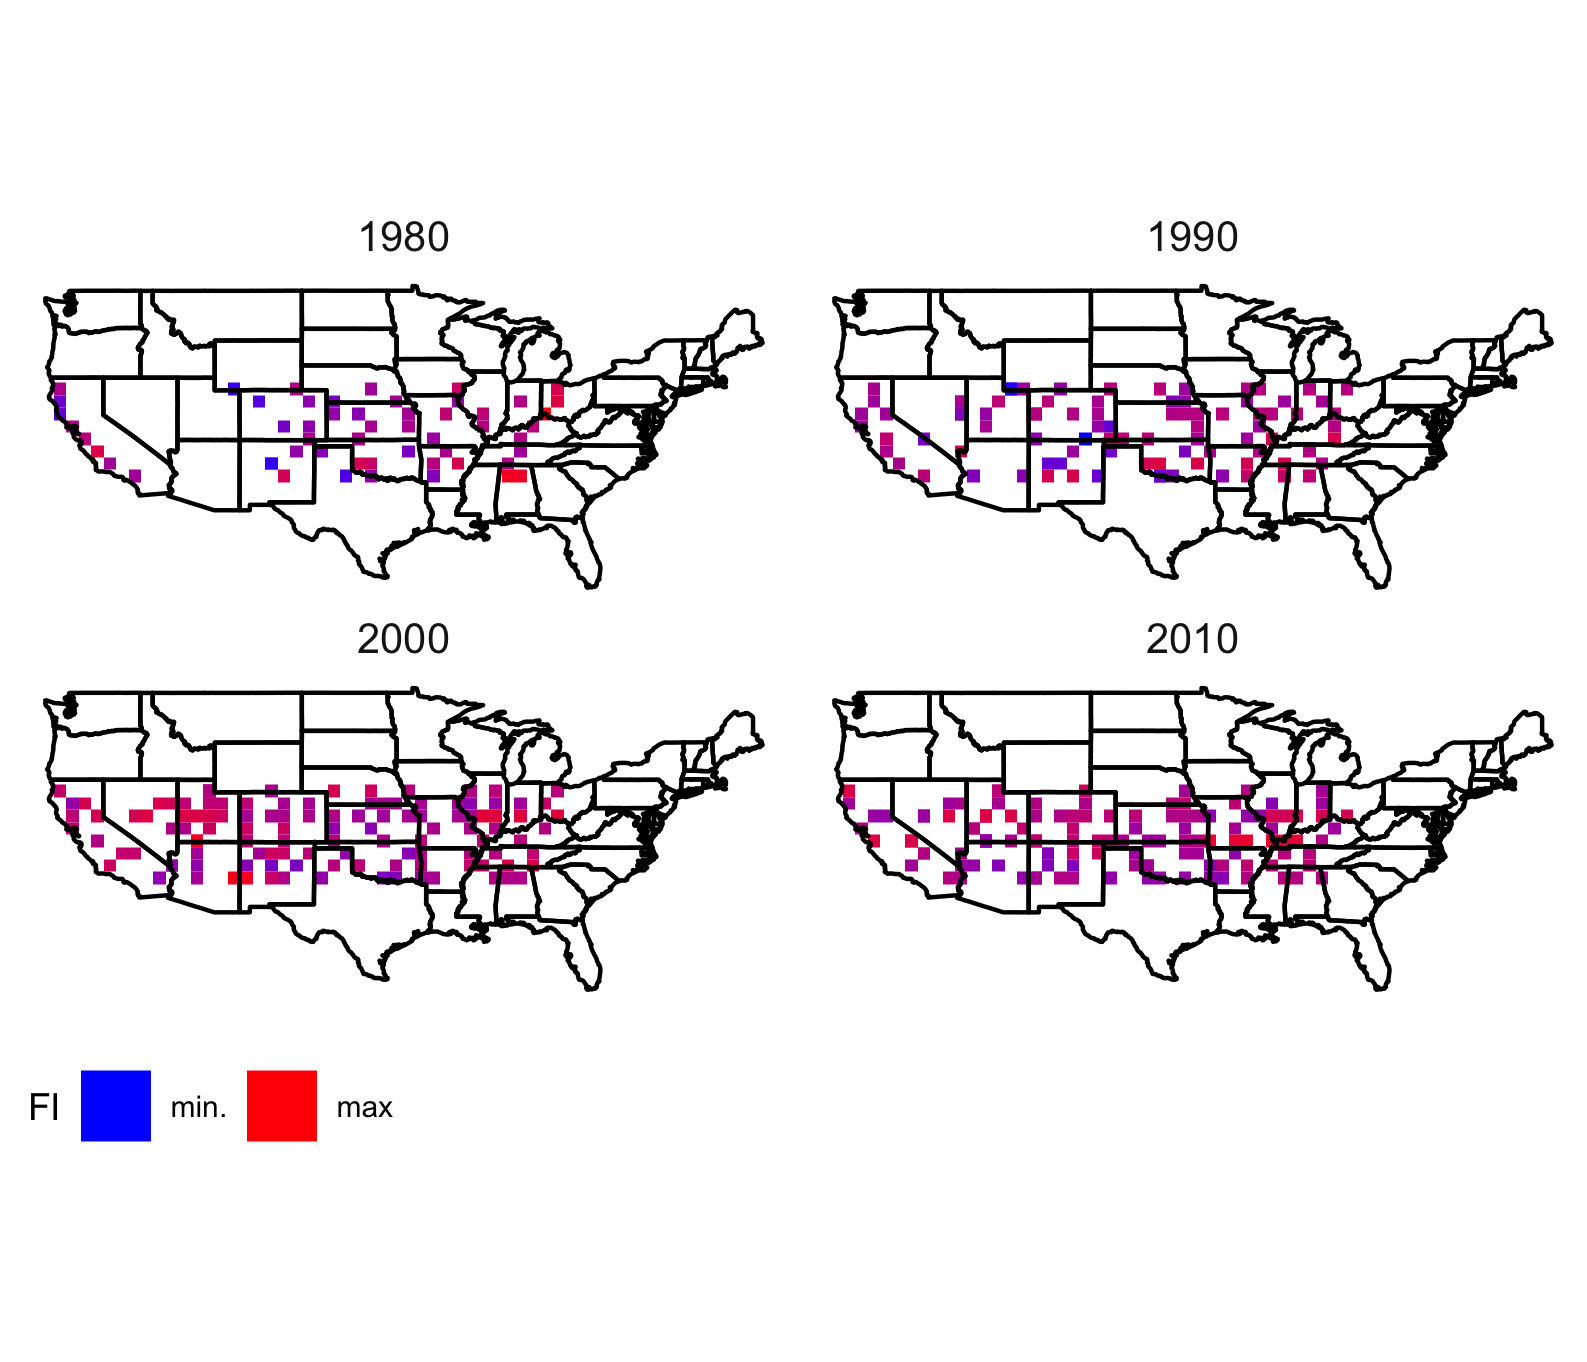
\includegraphics[width=0.95\linewidth]{./chapterFiles/fisherSpatial/figures/figsCalledInDiss/usaAllTsects_East-West_metric_logScaleFI} \caption{Fisher Information (top; log-scale bottom) of 5 East-West spatial transects over time. Adjacent changes of blue to red or vice-versa indicate regime shifts}\label{fig:usaFI}
\end{figure}
\subsection{Efficacy of Fisher Information as a spatial
RDM}\label{efficacy-of-fisher-information-as-a-spatial-rdm-1}

In addition to failing to identfiy clear geological boundaries across
large swaths of our study area (Fig.\ref{fig:usaFI}), I also did not
identify spatial correlation of Fisher Information among adjacent
spatial transects (Figs. \ref{fig:corPlotTsectsInterp},
\ref{fig:corPlotTsectsInterpLog}.
\begin{figure}
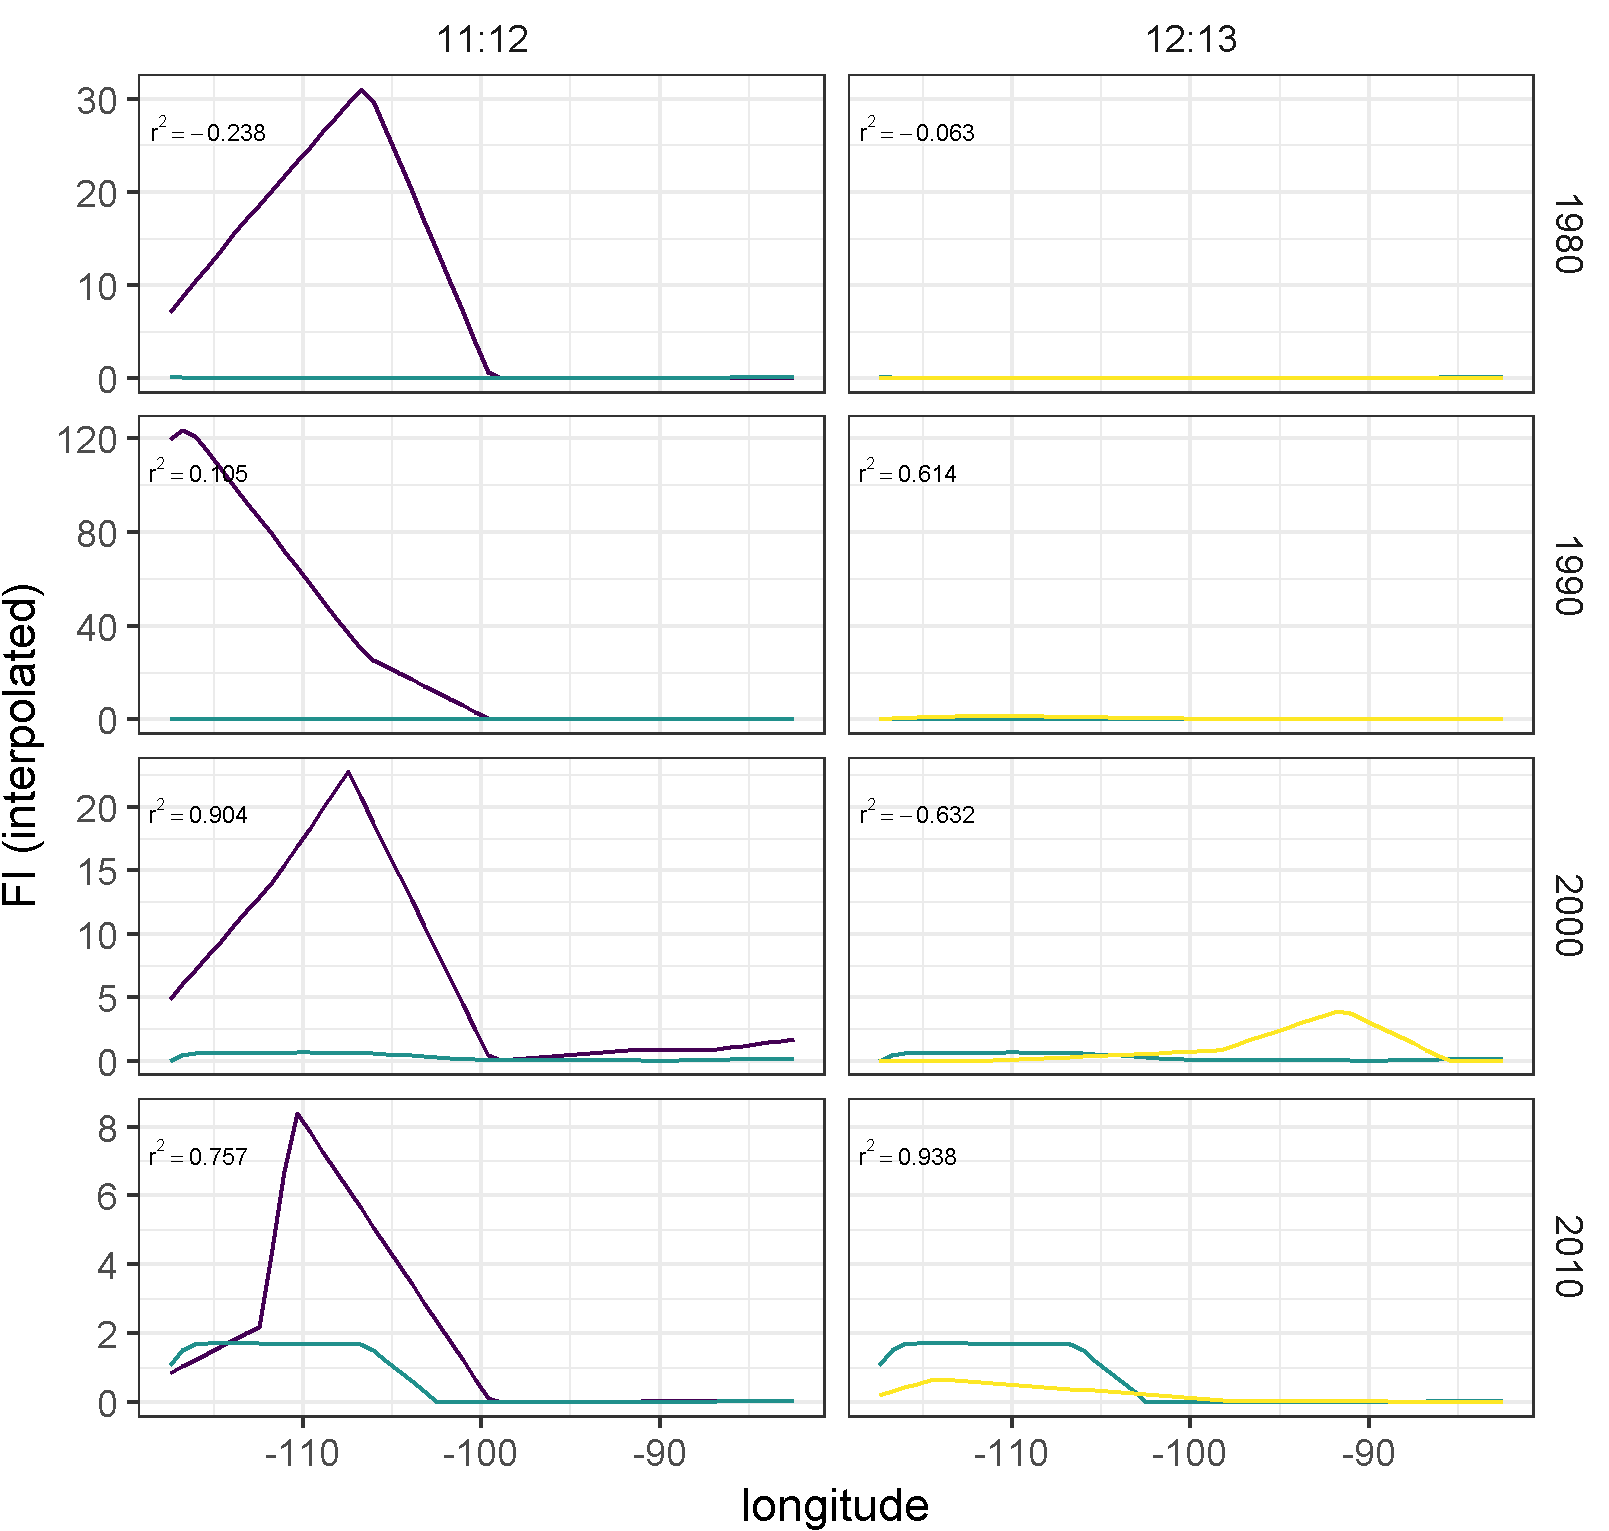
\includegraphics[width=0.95\linewidth]{./chapterFiles/fisherSpatial/figures/figsCalledInDiss/interpolated_FI_corplotSelectTransects_East-West} \caption{Pairwise relationships of Fisher Information (interpolated values) of spatially adjacent transects over time. Pairs were compared (column) at select sampling years (rows), and pair-wise correlations among paired transects are presented. Large, positive correlations indicate Fisher Information signals similarly at adjacent spatial transects.}\label{fig:corPlotTsectsInterp}
\end{figure}
\begin{figure}
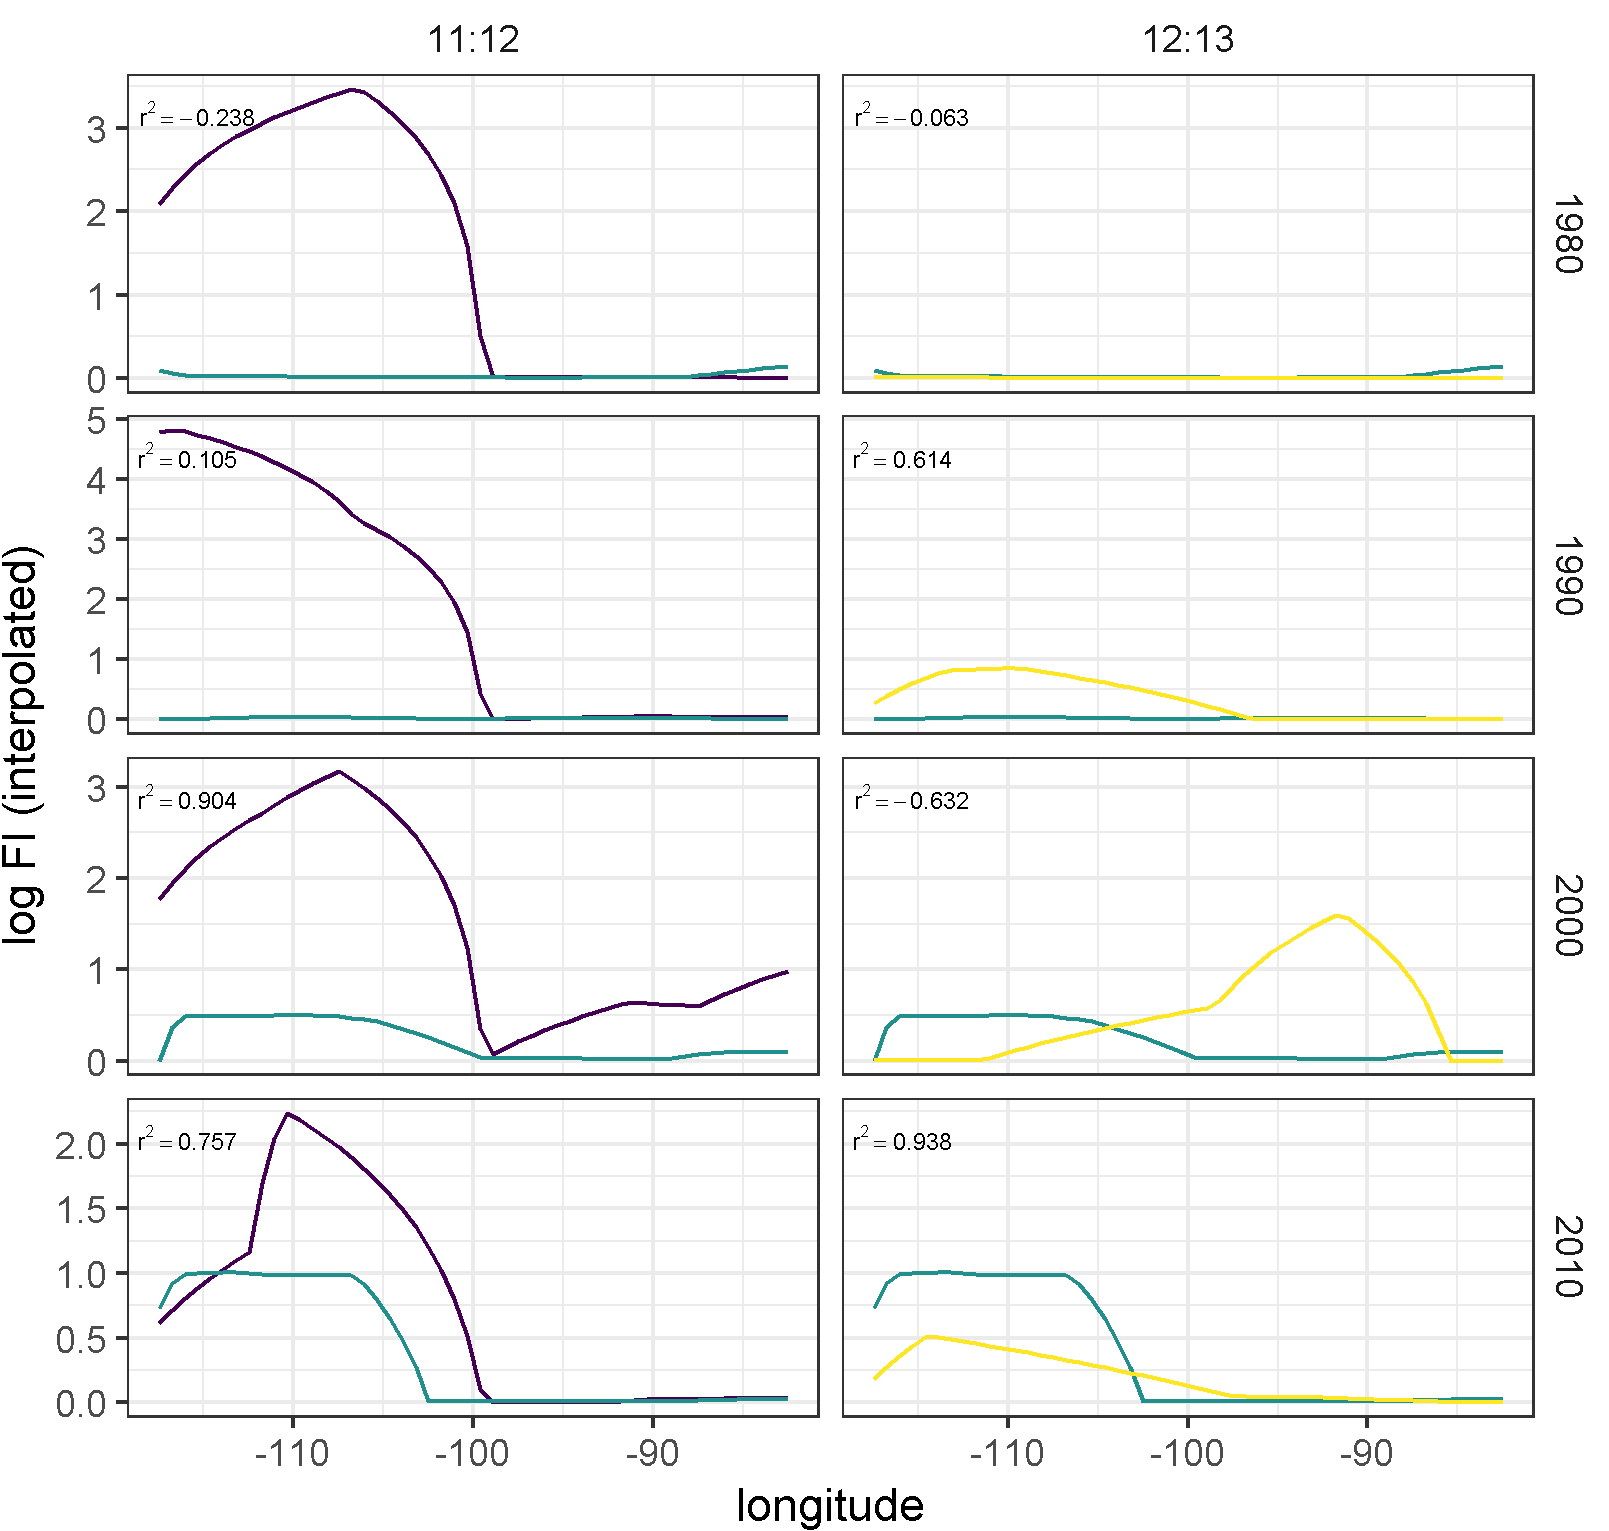
\includegraphics[width=0.95\linewidth]{./chapterFiles/fisherSpatial/figures/figsCalledInDiss/interpolated_FI_corplotSelectTransects_East-West_log} \caption{Pairwise relationships of Fisher Information (interpolated values on the log-scale) of spatially adjacent transects over time. Pairs were compared (column) at select sampling years (rows), and pair-wise correlations among paired transects are presented. Large, positive correlations indicate Fisher Information signals similarly at adjacent spatial transects.}\label{fig:corPlotTsectsInterpLog}
\end{figure}
\section{Discussion}\label{discussion-1}

The Fisher Information measure was introduced as a method to avoid some
analytical issues related to complex and noisy ecological data
(Karunanithi et al., 2008), and has also been suggested as an indicator
of \emph{spatial} regimes (Sundstrom et al., 2017a). I found no evidence
suggesting Fisher Information {[}Eq. \eqref{eq:derivativesFI}{]} can
identify `spatial regimes'. Further, the absence of autocorrelation
among spatially adjacent transects suggests Fisher Information may not
be a realiable indicator of changes in bird community structure.

Although the Fisher Information equation {[}Eq.
\eqref{eq:derivativesFI}{]} used in this study is a relatively
straightforward and fairly inexpensive computational calculation,
extreme care should be taken when applying this index to ecological
data. Fisher Information is capable of handling an infinite number of
inputs (variables), and given sufficiently low window size paramters,
can technically calculate an index value for only two observations. It
is important that the user understands the assumptions of identifying
'regime shifts; using Fisher Information, since the efficacy of this
method has not been yet subjected to rigorous tests (but see
@ref(???ResamplingCHapter???)). There are three primary assumptions
required when using Fisher Information to estimate relative orderliness
within ecological data (D. A. L. Mayer et al., 2007):\\
1. the order or state(s) (\(s\)) of the system is observable, 1. any
observable change in the information observed in the data represents
reality and the variables used in the analyses will not produce false
negatives, and 1. changes in \(I\) presumed to be regime shifts do not
represent the peaks of cyclic (periodic) patterns.

The first assumption is one of philosophical debate and is thus not
controllable. To attempt to control for false negatives, the user should
take caution in her choice of input variables. In the the case of a high
dimensional data, relativization and/or variable reduction measures may
be useful (Rodionov 2005). However, Fisher Information does not convey
information on how specific variables relate to the calculated index.
Finally, we can take measures to account for cyclic behavior in the data
by ensuring integration periods capture at one full cycle of the system
and, given sufficently high number of observations, increasing the
integration period may also alleviate some issues related to irreducible
error (white noise).

The lack of patterns identified using Fisher Information may be
influenced by one or more of the following: (1) the Breeding Bird Survey
data collection scheme was designed to estimate and track
\textbf{species} trends and not changes in entire communities; (2) these
data consist of \textless{} 50 time points, and for some BBS routes much
fewer. Ecological processes affecting large regions in this study area
(e.g., the Central Great Plains) operate on larger time scales (i.e.,
\textgreater{}\textgreater{} 50 points). A mismatch among the
ecologically relevant scales and the temporal resolution and extent of
our data may influence the ability of this index to capture large-scale
changes in whole bird communities.

Aside from the typical biases associated with the BBS data (e.g.,
species detection probability, observer bias), there are additional
considerations to be made when using these data to identify `spatial
regimes'. Breeding Bird Survey routes are spaced apart so as to reduce
the probability of observing the same individuals, but birds which fly
(especially in large flocks) overhead to foraging or roosting sites have
a higher probability of being detected on multiple routes. We have,
however, removed these species (waders, shorebirds, waterfowl, herons)
from analysis.

Regardless, this study assumes there is potential for each unique BBS
route to represent its own state. If routes were closer together, it is
more probable that the same type adn number of species would be
identified on adjacent routes. Therefore, if this method does not detect
slight changes in nearby routes which occupy the same `regime', then it
follows that the method is sensitive to loss or inclusion of new
species, which are spatially bounded by geological and vegetative
characteristics. What new information does this give us about the
system? Fisher Information reduces and removes the dimensionality of
these middle-numbered systems, which omits critical information.

Effective regime detection measures should provide sufficient evidence
of the drivers and/or pressures associated with the identified regime
shifts (Mac Nally, Albano, \& Fleishman, 2014). The Fisher Information
index collapses a wealth of data into a single metric, thereby foregoing
the ability to relate state variables to the observed changes in Fisher
Information, unlike other dimension reduction techniques. For example,
loadings, or the relative influence of variables on the ordinated axes,
can be derived from a Principal Components Analysis--this cannot be
achieved using Fisher Information. If Fisher Information clearly
suggested a spatial regime boundary or shift, a before-and-after
post-hoc analysis of the regional community dynamics might confirm the
regime shift occurrence.

Several questions remain regarding the efficacy of Fisher Information as
a regime detection measure in both spatial and temporal data. If signals
of regime shifts do exist, it is clearly not possible to identify them
using visual interpretation. I also did not find evidence to suggest
spatial autocorrelation of the calculations. I suggest future studies of
Fisher Infomration focuses on temporal, rather than spatial data.
Potential areas of research and questions include: 1. Relationship of
Fisher Information to likelihood ratio-based unsupervised change-point
detection algorithms (e.g., ChangeFinder (Liu, Yamada, Collier, \&
Sugiyama, 2013)). 1. Sensitivity of Fisher Information to data quality
and quantity {[}this is explored in Chapter \ref{resampling}{]}. 1.
What, if any, advantages does FI have over other density estimation
techniques?\\
1. Does FI provide signals in addition to or different than geophysical
and vegetative (e.g.~LIDAR) observations (data)?

\chapter{Distance travelled}\label{distanceTravelled}

\section{Introduction}\label{introduction-3}

Defining a regime shift

There are different types fo regime shifts, and \textbf{why those
differences matter}
\begin{itemize}
\tightlist
\item
  only ???regime shifts??? that are also ???critical transitions???
  should show ???critical slowing down???
  \begin{itemize}
  \tightlist
  \item
    so that???s an important \emph{technical distinction} if you???re
    trying to use \emph{???early warning signals???}.\\
  \end{itemize}
\item
  There are mutiple types og \textbf{critical transitions}
  \begin{itemize}
  \tightlist
  \item
    these results in very different changes in time series\\
  \item
    in some contexts, this doesn't really matter
  \end{itemize}
\end{itemize}
\section{Methodology}\label{methodology}

\section{Case study}\label{case-study-1}

\section{Discussion}\label{discussion-2}

\chapter*{Appendix A}\label{rRDM}
\addcontentsline{toc}{chapter}{Appendix A}

Placeholder

\chapter*{Catch-all, unused, to be removed from
pdf}\label{catch-all-unused-to-be-removed-from-pdf}
\addcontentsline{toc}{chapter}{Catch-all, unused, to be removed from
pdf}

Placeholder

\section{Random}\label{random}

\section{On the complexity of nature}\label{on-the-complexity-of-nature}

\section{On analysing ecol time series
data}\label{on-analysing-ecol-time-series-data}

\section{on improving RDMs}\label{on-improving-rdms}

\section{on fisher info}\label{on-fisher-info}

\section{On the evidence for ecol regime
shifts}\label{on-the-evidence-for-ecol-regime-shifts}

\section{On alternative stable
staets}\label{on-alternative-stable-staets}

\section{On critical slowing down}\label{on-critical-slowing-down}

\section{Brandolini's principle}\label{brandolinis-principle}

\section{Importance of this thesis}\label{importance-of-this-thesis}

\section{Some notes on RSDMs not yet in
text.}\label{some-notes-on-rsdms-not-yet-in-text.}

\section{This section contains notes on model-based and metric-based
methods for detecting regime
shifts}\label{this-section-contains-notes-on-model-based-and-metric-based-methods-for-detecting-regime-shifts}

\section{Types of regime dtection
methods}\label{types-of-regime-dtection-methods}

\subsection{Model-based}\label{model-based}

\subsection{Metric-based}\label{metric-based}

\section{Some text from the review chapter
-}\label{some-text-from-the-review-chapter--}

\section{FISHER BININNGIN SHIT}\label{fisher-bininngin-shit}

\section{Unused text}\label{unused-text}

\subsection{Issues with usign the BBS
data}\label{issues-with-usign-the-bbs-data}

\subsection{How are RDMs useful to ecological
management?}\label{how-are-rdms-useful-to-ecological-management}

\section{For resampling chapter}\label{for-resampling-chapter}

\chapter*{References}\label{references}
\addcontentsline{toc}{chapter}{References}

Placeholder

\hypertarget{refs}{}
\hypertarget{ref-bestelmeyer_analysis_2011}{}
Bestelmeyer, B. T., Ellison, A. M., Fraser, W. R., Gorman, K. B.,
Holbrook, S. J., Laney, C. M., \ldots{} others. (2011). Analysis of
abrupt transitions in ecological systems. \emph{Ecosphere},
\emph{2}(12), 1--26.

\hypertarget{ref-brock_variance_2006}{}
Brock, W., \& Carpenter, S. (2006). Variance as a Leading Indicator of
Regime Shift in Ecosystem Services. \emph{Ecology and Society},
\emph{11}(2). \url{http://doi.org/10.5751/ES-01777-110209}

\hypertarget{ref-butitta_spatial_2017}{}
Butitta, V. L., Carpenter, S. R., Loken, L. C., Pace, M. L., \& Stanley,
E. H. (2017). Spatial early warning signals in a lake manipulation.
\emph{Ecosphere}, \emph{8}(10), n/a--n/a.
\url{http://doi.org/10.1002/ecs2.1941}

\hypertarget{ref-deangelis2017spatially}{}
DeAngelis, D. L., \& Yurek, S. (2017). Spatially explicit modeling in
ecology: A review. \emph{Ecosystems}, \emph{20}(2), 284--300.

\hypertarget{ref-dutta2018robustness}{}
Dutta, P. S., Sharma, Y., \& Abbott, K. C. (2018). Robustness of early
warning signals for catastrophic and non-catastrophic transitions.
\emph{Oikos}, \emph{127}(9), 1251--1263.

\hypertarget{ref-eason_evaluating_2012}{}
Eason, T., \& Cabezas, H. (2012). Evaluating the sustainability of a
regional system using Fisher information in the San Luis Basin,
Colorado. \emph{Journal of Environmental Management}, \emph{94}(1),
41--49.

\hypertarget{ref-fath_regime_2003}{}
Fath, B. D., Cabezas, H., \& Pawlowski, C. W. (2003). Regime changes in
ecological systems: An information theory approach. \emph{Journal of
Theoretical Biology}, \emph{222}(4), 517--530.
\url{http://doi.org/10.1016/S0022-5193(03)00067-5}

\hypertarget{ref-karunanithi_detection_2008}{}
Karunanithi, A. T., Cabezas, H., Frieden, B. R., \& Pawlowski, C. W.
(2008). Detection and assessment of ecosystem regime shifts from fisher
information. \emph{Ecology and Society}, \emph{13}(1).

\hypertarget{ref-kefi2014early}{}
Kefi, S., Guttal, V., Brock, W. A., Carpenter, S. R., Ellison, A. M.,
Livina, V. N., \ldots{} Dakos, V. (2014). Early warning signals of
ecological transitions: Methods for spatial patterns. \emph{PloS One},
\emph{9}(3), e92097.

\hypertarget{ref-liu2013change}{}
Liu, S., Yamada, M., Collier, N., \& Sugiyama, M. (2013). Change-point
detection in time-series data by relative density-ratio estimation.
\emph{Neural Networks}, \emph{43}, 72--83.

\hypertarget{ref-mac2014scrutiny}{}
Mac Nally, R., Albano, C., \& Fleishman, E. (2014). A scrutiny of the
evidence for pressure-induced state shifts in estuarine and nearshore
ecosystems. \emph{Austral Ecology}, \emph{39}(8), 898--906.

\hypertarget{ref-mayer_fisher_2006}{}
Mayer, A. L., Pawlowski, C. W., \& Cabezas, H. (2006). Fisher
Information and dynamic regime changes in ecological systems.
\emph{Ecological Modelling}, \emph{195}(1???2), 72--82.
\url{http://doi.org/10.1016/j.ecolmodel.2005.11.011}

\hypertarget{ref-mayer_applications_2007}{}
Mayer, D. A. L., Pawlowski, D. C., Fath, P. B. D., \& Cabezas, D. H.
(2007). Applications of Fisher Information to the Management of
Sustainable Environmental Systems. In B. R. F. B. MS \& R. A. G. B. MD
(Eds.), \emph{Exploratory Data Analysis Using Fisher Information} (pp.
217--244). Springer London.
\url{http://doi.org/10.1007/978-1-84628-777-0_7}

\hypertarget{ref-perretti2012regime}{}
Perretti, C. T., \& Munch, S. B. (2012). Regime shift indicators fail
under noise levels commonly observed in ecological systems.
\emph{Ecological Applications}, \emph{22}(6), 1772--1779.

\hypertarget{ref-sundstrom_detecting_2017}{}
Sundstrom, S. M., Eason, T., Nelson, R. J., Angeler, D. G., Barichievy,
C., Garmestani, A. S., \ldots{} Knutson, M. (2017a). Detecting spatial
regimes in ecosystems. \emph{Ecology Letters}, \emph{20}(1), 19--32.

\hypertarget{ref-sundstrom2017detecting}{}
Sundstrom, S. M., Eason, T., Nelson, R. J., Angeler, D. G., Barichievy,
C., Garmestani, A. S., \ldots{} Allen, C. R. (2017b). Detecting spatial
regimes in ecosystems. \emph{Ecology Letters}, \emph{20}(1), 19--32.
\url{http://doi.org/10.1111/ele.12709}


\end{document}
